%
% File acl2021.tex
%
%% Based on the style files for EMNLP 2020, which were
%% Based on the style files for ACL 2020, which were
%% Based on the style files for ACL 2018, NAACL 2018/19, which were
%% Based on the style files for ACL-2015, with some improvements
%%  taken from the NAACL-2016 style
%% Based on the style files for ACL-2014, which were, in turn,
%% based on ACL-2013, ACL-2012, ACL-2011, ACL-2010, ACL-IJCNLP-2009,
%% EACL-2009, IJCNLP-2008...
%% Based on the style files for EACL 2006 by 
%%e.agirre@ehu.es or Sergi.Balari@uab.es
%% and that of ACL 08 by Joakim Nivre and Noah Smith

\documentclass[11pt,a4paper]{article}
\usepackage[hyperref]{acl2021}
\usepackage{times}
\usepackage{latexsym}
\usepackage{graphicx}
\usepackage{CJKutf8}
\usepackage{amsmath}
\usepackage{bm}
\usepackage{booktabs}
\usepackage{multirow}
\usepackage{url}
\usepackage{breakurl}

% ADD FOR PICT
\usepackage{tikz-dependency}
\usepackage{amsmath}
\usepackage{graphicx}
\usepackage{pgfplots}
\usepackage{tikz}
\usepackage[center]{subfigure}
\usepackage{tikz-qtree}
\usepgflibrary{arrows.meta}
\usepgfplotslibrary{fillbetween}
\usetikzlibrary{fit, calc, decorations.pathreplacing, positioning, shapes.geometric, backgrounds}
\usepackage{float}
% ADD FOR PICT END

\def\UrlBreaks{\do\/\do-}

\renewcommand{\UrlFont}{\ttfamily\small}

% This is not strictly necessary, and may be commented out,
% but it will improve the layout of the manuscript,
% and will typically save some space.
\usepackage{microtype}

\aclfinalcopy % Uncomment this line for the final submission
\def\aclpaperid{2185} %  Enter the acl Paper ID here

%\setlength\titlebox{5cm}
% You can expand the titlebox if you need extra space
% to show all the authors. Please do not make the titlebox
% smaller than 5cm (the original size); we will check this
% in the camera-ready version and ask you to change it back.

\newcommand\BibTeX{B\textsc{ib}\TeX}

\title{
%An In-depth 
% Study on Deep Syntactic Char-level Structures of Chinese Words
% An In-depth Study on Char-level Syntactic Structure of Chinese Words
An In-depth Study on Internal Structure of Chinese Words
}

\author{
Chen Gong$^{1}$, Saihao Huang$^1$\thanks{$~$ Chen Gong and Saihao Huang make equal contributions to this
work. Zhenghua is the corresponding author.}, Houquan Zhou$^1$, Zhenghua Li$^1$, Min Zhang$^1$,\\ {\bf Zhefeng Wang}$^2$, {\bf Baoxing Huai}$^2$, {\bf Nicholas Jing Yuan}$^2$ \\
$^1$Institute of Artificial Intelligence, School of Computer Science and Technology, \\Soochow University, China; $~~~~~$
$^2$ Huawei Cloud, China  \\
{\tt $^1$\{cgong,shhuang1999,hqzhou\}@stu.suda.edu.cn} \\
{\tt $^1$\{zhli13,minzhang\}@suda.edu.cn} \\
{\tt $^2$\{wangzhefeng, huaibaoxing, nicholas.yuan\}@huawei.com} \\
}


\date{}

\begin{document}
\maketitle
\begin{CJK}{UTF8}{gkai}
  In this paper, we explore the connection between secret key agreement and secure omniscience within the setting of the multiterminal source model with a wiretapper who has side information. While the secret key agreement problem considers the generation of a maximum-rate secret key through public discussion, the secure omniscience problem is concerned with communication protocols for omniscience that minimize the rate of information leakage to the wiretapper. The starting point of our work is a lower bound on the minimum leakage rate for omniscience, $\rl$, in terms of the wiretap secret key capacity, $\wskc$. Our interest is in identifying broad classes of sources for which this lower bound is met with equality, in which case we say that there is a duality between secure omniscience and secret key agreement. We show that this duality holds in the case of certain finite linear source (FLS) models, such as two-terminal FLS models and pairwise independent network models on trees with a linear wiretapper. Duality also holds for any FLS model in which $\wskc$ is achieved by a perfect linear secret key agreement scheme. We conjecture that the duality in fact holds unconditionally for any FLS model. On the negative side, we give an example of a (non-FLS) source model for which duality does not hold if we limit ourselves to communication-for-omniscience protocols with at most two (interactive) communications.  We also address the secure function computation problem and explore the connection between the minimum leakage rate for computing a function and the wiretap secret key capacity.
  
%   Finally, we demonstrate the usefulness of our lower bound on $\rl$ by using it to derive equivalent conditions for the positivity of $\wskc$ in the multiterminal model. This extends a recent result of Gohari, G\"{u}nl\"{u} and Kramer (2020) obtained for the two-user setting.
  
   
%   In this paper, we study the problem of secret key generation through an omniscience achieving communication that minimizes the 
%   leakage rate to a wiretapper who has side information in the setting of multiterminal source model.  We explore this problem by deriving a lower bound on the wiretap secret key capacity $\wskc$ in terms of the minimum leakage rate for omniscience, $\rl$. 
%   %The former quantity is defined to be the maximum secret key rate achievable, and the latter one is defined as the minimum possible leakage rate about the source through an omniscience scheme to a wiretapper. 
%   The main focus of our work is the characterization of the sources for which the lower bound holds with equality \textemdash it is referred to as a duality between secure omniscience and wiretap secret key agreement. For general source models, we show that duality need not hold if we limit to the communication protocols with at most two (interactive) communications. In the case when there is no restriction on the number of communications, whether the duality holds or not is still unknown. However, we resolve this question affirmatively for two-user finite linear sources (FLS) and pairwise independent networks (PIN) defined on trees, a subclass of FLS. Moreover, for these sources, we give a single-letter expression for $\wskc$. Furthermore, in the direction of proving the conjecture that duality holds for all FLS, we show that if $\wskc$ is achieved by a \emph{perfect} secret key agreement scheme for FLS then the duality must hold. All these results mount up the evidence in favor of the conjecture on FLS. Moreover, we demonstrate the usefulness of our lower bound on $\wskc$ in terms of $\rl$ by deriving some equivalent conditions on the positivity of secret key capacity for multiterminal source model. Our result indeed extends the work of Gohari, G\"{u}nl\"{u} and Kramer in two-user case.
% \leavevmode
% \\
% \\
% \\
% \\
% \\
\section{Introduction}
\label{introduction}

AutoML is the process by which machine learning models are built automatically for a new dataset. Given a dataset, AutoML systems perform a search over valid data transformations and learners, along with hyper-parameter optimization for each learner~\cite{VolcanoML}. Choosing the transformations and learners over which to search is our focus.
A significant number of systems mine from prior runs of pipelines over a set of datasets to choose transformers and learners that are effective with different types of datasets (e.g. \cite{NEURIPS2018_b59a51a3}, \cite{10.14778/3415478.3415542}, \cite{autosklearn}). Thus, they build a database by actually running different pipelines with a diverse set of datasets to estimate the accuracy of potential pipelines. Hence, they can be used to effectively reduce the search space. A new dataset, based on a set of features (meta-features) is then matched to this database to find the most plausible candidates for both learner selection and hyper-parameter tuning. This process of choosing starting points in the search space is called meta-learning for the cold start problem.  

Other meta-learning approaches include mining existing data science code and their associated datasets to learn from human expertise. The AL~\cite{al} system mined existing Kaggle notebooks using dynamic analysis, i.e., actually running the scripts, and showed that such a system has promise.  However, this meta-learning approach does not scale because it is onerous to execute a large number of pipeline scripts on datasets, preprocessing datasets is never trivial, and older scripts cease to run at all as software evolves. It is not surprising that AL therefore performed dynamic analysis on just nine datasets.

Our system, {\sysname}, provides a scalable meta-learning approach to leverage human expertise, using static analysis to mine pipelines from large repositories of scripts. Static analysis has the advantage of scaling to thousands or millions of scripts \cite{graph4code} easily, but lacks the performance data gathered by dynamic analysis. The {\sysname} meta-learning approach guides the learning process by a scalable dataset similarity search, based on dataset embeddings, to find the most similar datasets and the semantics of ML pipelines applied on them.  Many existing systems, such as Auto-Sklearn \cite{autosklearn} and AL \cite{al}, compute a set of meta-features for each dataset. We developed a deep neural network model to generate embeddings at the granularity of a dataset, e.g., a table or CSV file, to capture similarity at the level of an entire dataset rather than relying on a set of meta-features.
 
Because we use static analysis to capture the semantics of the meta-learning process, we have no mechanism to choose the \textbf{best} pipeline from many seen pipelines, unlike the dynamic execution case where one can rely on runtime to choose the best performing pipeline.  Observing that pipelines are basically workflow graphs, we use graph generator neural models to succinctly capture the statically-observed pipelines for a single dataset. In {\sysname}, we formulate learner selection as a graph generation problem to predict optimized pipelines based on pipelines seen in actual notebooks.

%. This formulation enables {\sysname} for effective pruning of the AutoML search space to predict optimized pipelines based on pipelines seen in actual notebooks.}
%We note that increasingly, state-of-the-art performance in AutoML systems is being generated by more complex pipelines such as Directed Acyclic Graphs (DAGs) \cite{piper} rather than the linear pipelines used in earlier systems.  
 
{\sysname} does learner and transformation selection, and hence is a component of an AutoML systems. To evaluate this component, we integrated it into two existing AutoML systems, FLAML \cite{flaml} and Auto-Sklearn \cite{autosklearn}.  
% We evaluate each system with and without {\sysname}.  
We chose FLAML because it does not yet have any meta-learning component for the cold start problem and instead allows user selection of learners and transformers. The authors of FLAML explicitly pointed to the fact that FLAML might benefit from a meta-learning component and pointed to it as a possibility for future work. For FLAML, if mining historical pipelines provides an advantage, we should improve its performance. We also picked Auto-Sklearn as it does have a learner selection component based on meta-features, as described earlier~\cite{autosklearn2}. For Auto-Sklearn, we should at least match performance if our static mining of pipelines can match their extensive database. For context, we also compared {\sysname} with the recent VolcanoML~\cite{VolcanoML}, which provides an efficient decomposition and execution strategy for the AutoML search space. In contrast, {\sysname} prunes the search space using our meta-learning model to perform hyperparameter optimization only for the most promising candidates. 

The contributions of this paper are the following:
\begin{itemize}
    \item Section ~\ref{sec:mining} defines a scalable meta-learning approach based on representation learning of mined ML pipeline semantics and datasets for over 100 datasets and ~11K Python scripts.  
    \newline
    \item Sections~\ref{sec:kgpipGen} formulates AutoML pipeline generation as a graph generation problem. {\sysname} predicts efficiently an optimized ML pipeline for an unseen dataset based on our meta-learning model.  To the best of our knowledge, {\sysname} is the first approach to formulate  AutoML pipeline generation in such a way.
    \newline
    \item Section~\ref{sec:eval} presents a comprehensive evaluation using a large collection of 121 datasets from major AutoML benchmarks and Kaggle. Our experimental results show that {\sysname} outperforms all existing AutoML systems and achieves state-of-the-art results on the majority of these datasets. {\sysname} significantly improves the performance of both FLAML and Auto-Sklearn in classification and regression tasks. We also outperformed AL in 75 out of 77 datasets and VolcanoML in 75  out of 121 datasets, including 44 datasets used only by VolcanoML~\cite{VolcanoML}.  On average, {\sysname} achieves scores that are statistically better than the means of all other systems. 
\end{itemize}


%This approach does not need to apply cleaning or transformation methods to handle different variances among datasets. Moreover, we do not need to deal with complex analysis, such as dynamic code analysis. Thus, our approach proved to be scalable, as discussed in Sections~\ref{sec:mining}.
\section{Related Work}\label{sec:related}
 
The authors in \cite{humphreys2007noncontact} showed that it is possible to extract the PPG signal from the video using a complementary metal-oxide semiconductor camera by illuminating a region of tissue using through external light-emitting diodes at dual-wavelength (760nm and 880nm).  Further, the authors of  \cite{verkruysse2008remote} demonstrated that the PPG signal can be estimated by just using ambient light as a source of illumination along with a simple digital camera.  Further in \cite{poh2011advancements}, the PPG waveform was estimated from the videos recorded using a low-cost webcam. The red, green, and blue channels of the images were decomposed into independent sources using independent component analysis. One of the independent sources was selected to estimate PPG and further calculate HR, and HRV. All these works showed the possibility of extracting PPG signals from the videos and proved the similarity of this signal with the one obtained using a contact device. Further, the authors in \cite{10.1109/CVPR.2013.440} showed that heart rate can be extracted from features from the head as well by capturing the subtle head movements that happen due to blood flow.

%
The authors of \cite{kumar2015distanceppg} proposed a methodology that overcomes a challenge in extracting PPG for people with darker skin tones. The challenge due to slight movement and low lighting conditions during recording a video was also addressed. They implemented the method where PPG signal is extracted from different regions of the face and signal from each region is combined using their weighted average making weights different for different people depending on their skin color. 
%

There are other attempts where authors of \cite{6523142,6909939, 7410772, 7412627} have introduced different methodologies to make algorithms for estimating pulse rate robust to illumination variation and motion of the subjects. The paper \cite{6523142} introduces a chrominance-based method to reduce the effect of motion in estimating pulse rate. The authors of \cite{6909939} used a technique in which face tracking and normalized least square adaptive filtering is used to counter the effects of variations due to illumination and subject movement. 
The paper \cite{7410772} resolves the issue of subject movement by choosing the rectangular ROI's on the face relative to the facial landmarks and facial landmarks are tracked in the video using pose-free facial landmark fitting tracker discussed in \cite{yu2016face} followed by the removal of noise due to illumination to extract noise-free PPG signal for estimating pulse rate. 

Recently, the use of machine learning in the prediction of health parameters have gained attention. The paper \cite{osman2015supervised} used a supervised learning methodology to predict the pulse rate from the videos taken from any off-the-shelf camera. Their model showed the possibility of using machine learning methods to estimate the pulse rate. However, our method outperforms their results when the root mean squared error of the predicted pulse rate is compared. The authors in \cite{hsu2017deep} proposed a deep learning methodology to predict the pulse rate from the facial videos. The researchers trained a convolutional neural network (CNN) on the images generated using Short-Time Fourier Transform (STFT) applied on the R, G, \& B channels from the facial region of interests.
The authors of \cite{osman2015supervised, hsu2017deep} only predicted pulse rate, and we extended our work in predicting variance in the pulse rate measurements as well.

All the related work discussed above utilizes filtering and digital signal processing to extract PPG signals from the video which is further used to estimate the PR and PRV.  %
The method proposed in \cite{kumar2015distanceppg} is person dependent since the weights will be different for people with different skin tone. In contrast, we propose a deep learning model to predict the PR which is independent of the person who is being trained. Thus, the model would work even if there is no prior training model built for that individual and hence, making our model robust. 

%


\section{Word-internal Structure Annotation}\label{sec:data-annotation}
%Intra-Word Character Dependency Treebank (IWDT)}

In this section, we describe in detail the annotation process of WIST. 
As shown in Figure \ref{fig:example}-(c), we adopt dependency trees for representing word-internal structure. 
The reason is two-fold. First, word-formation process correlates with syntax in different ways depending on language type \cite{Aikhenvald-2007-typological}. Such correlation is especially close for Chinese due to its lack of morphological inflections. In particular, \citet{grammar-notes-zhu-1982} presented thorough  investigation on Chinese word formation mainly from a syntactic view. 
Second, as a grammar formalism, dependency tree structure has been widely adopted for capturing sentence-level syntax due to its simplicity and flexibility in representing  relations. Meanwhile, its computational modeling is also developed quite well. 
%我们为什么采用依存树的形式?首先,汉语词内部结构本身和句法紧密相关,给出参考文献。第二,依存句法树形式,是近年来最流行的句法表示方法,多语言使用。主要就在于可以用label来区分组合的模式。




% 传统的人工标注数据通常以词为基本的syntactic unit, such as CTB, PKU, MSR, 
% This form of annotation does not
% give character-level syntactic structures for words,
% a source of linguistic information that is more fundamental
% and less sparse than atomic words.

% Considering that a word is defined by all the characters inside that subtly interact with each other from both syntax and semantics.
% Unlike alphabetical languages, Chinese
% characters convey meanings, and the meaning of
% most Chinese words takes roots in their character.a series of work因此一些工作开始标注词内部结构【引用】。most of the previous annotations通常只考虑内部结构框架或者核心字的位置,忽略了词内部各constituent unit之间的关系。Zhao 通过combine character-level POS tag来表示dependency label.然而这种表示不能直观地展示出各个字直接的主谓宾定状补关系。
% To overcome this obstacle, we construct一个词内部结构数据集according to our newly complied annotation guideline, which contains 11种依存关系,能够更直观地表达。。。

% Traditional manually annotated Chinese corpus such as CTB【】, PKU【】 and MSR【】 usually take words as the basic units, neglecting the character-level intra-word structures. In fact, the way that the Chinese characters inside the words interact with each other can convey meanings from the perspective of both syntax and semantic. In order to make use of the linguistic information from the internal word structure, several recent work has annotated constituent or dependency style internal structures for words【参考文献】. Most of these work mainly focus on the the hierarchical structure or the head character information for each word, without considering the relation types between constituent characters inside the word.
% % composition architecture 【意思是只关注框架结构,怎么写】 or the position of the head character for words, without considering the relation types between the constituent characters inside the words.
% 【Zhao】 represent intra-word character-level dependency label by combining the character-level POS tags of the constituent characters. However, the typical syntactic structures such as subject-predicate, verb-object, modifier-noun, coordination, which is quite important for analyzing。。。  can not be directly reflected by such dependency labels.
% To overcome this obstacle, we construct intra-word character dependency treebank of over xxx words CTB5 \cite{xue2005ctb} and CoNLL09 \cite{conll09} according to our newly complied annotation guideline, which contains 11 relations to intuitively reflect the internal dependency syntax for Chinese words.

% 什么是词内部结构?
% 为什么要标注词内部结构?
% 前人是怎么标注词内部结构的?
% 我们相比之下的优势?
% 可以给出图比较

%\subsection{Annotation Process}

\paragraph{Annotation guidelines.} 
After several months' survey,  we have compiled  systematic and detailed
 guidelines for word-internal structure annotation. 
Our guidelines are mainly based on the famous textbook on Chinese grammar of \citet{grammar-notes-zhu-1982}. 
We intensively studied all previous works on word-internal structure annotation, which are discussed in Section \ref{sec:related-work}.
We also find that it is quite beneficial to be familiar with guidelines developed by previous annotation projects for Chinese word segmentation \cite{ctb-xiafei,yu2003ppd}.

% 感觉没有说到重点。我们的规范,主要参考的了哪些资料?
% 语法讲义:稍微细致的展开一下。
% 汉语构词:

% Given an input word, annotators are asked to annotate the dependency arcs and the corresponding relation labels between the characters to capture the intra-word syntactic structure.
% The role of the IWDT annotation guideline is to provide the annotation rules of 
% intra-word syntax structures under various linguist phenomena for annotators' reference.
%After a few months' in-depth study,  we have compiled a systematic and detailed
%annotation guideline for Chinese intra-Word character dependency treebank construction. 

Our guidelines contain 11 relations specifically designed to capture the internal dependency syntax for Chinese words, as shown in Table \ref{tbl:summary-relation}. 
We derive most of the dependency relations by referring to guidelines of three popular Chinese dependency treebanks, i.e., UD, Harbin Institute Technology Chinese Dependency Treebank (HIT-CDT) \cite{HIT-CDT}, and Chinese Open Dependency Treebank (CODT) \cite{li-etal-2019-semi-supervised}. 
We give very detailed illustrations with examples in our 30-page guidelines to ensure annotation consistency and quality. 
Our guidelines are also gradually improved according to the feedback from the annotators. 
% The latest version is attached as supplementary material. 

\paragraph{Quality control.} 
We employ 18 undergraduate students as part-time annotators who are familiar with Chinese syntax, and select 6 capable annotators with a lot of data annotation experience as expert annotators 
to handle inconsistent submissions. %Before formal annotation
All the annotators (including expert annotators) were paid for their work . 
The salary is determined by both quantity and quality. Besides, we give extra bonus to the annotators with high accuracy. The average salary of the annotators is 30 RMB per hour.
% (a part-time waiter in KFC earns 20 RMB per hour in our city).
All annotators are trained %We train annotators 
for several hours to be familiar with our guidelines and the usage of annotation tool. 
% During formal annotation, annotators are encouraged to look up the guideline or use search engine for difficult or incomprehensible inputs, but are not allowed to discuss with each other, in order to guarantee quality.

We apply strict double annotation in order to guarantee quality. % of the labeled data. 
Each word 
% (without any word inputs) 
is randomly assigned to two annotators. Two identical submissions are directly used as the final answer. Otherwise, a third expert annotator is asked to decide the final answer after analyzing the two inconsistent annotations. 

\paragraph{Annotation tool.} 
We build a browser-based annotation tool to support the annotation workflow and facilitate project management.
% ,  which is also illustrated in detail in our supplementary material. 

%In the annotation interface, present all its POS tags to annotators. 
Given an annotation task, all its POS tags \footnote{In CTB5, a word may be annotated with different POS tags under different contexts. For example, ``发展 (development)'' is annotated as NN (noun) in the context ``促进经济发展 (boost the economic development )'', whereas ``发展 (develop)'' is annotated as (VV) verb in the context ``稳定地发展 (develop steadily)''. Therefore, when annotating the word ``发展 (develop/development )'', we present both ``noun'' and ``verb'' to the annotators for reference.''} of the focused word in CTB5 are presented to the annotator, in order to explore multiple internal structures for one word. 
In that case, the annotator can click a checkbox to inform us for further process. 
Please note that the manually annotated POS tags in CTB5 are converted into Universal Dependencies (UD) \footnote{\scriptsize{\url{universaldependencies.org/u/pos/}}} POS tags based on predefined mapping rules, since the original CTB5 POS tags are too fine-grained (33 tags) and difficult for annotators to understand.
The interface also presents several example sentences to improve annotation efficiency. We strongly encourage annotators to look up difficult words or characters in electronic dictionaries.\footnote{Eg., \url{hanyu.baidu.com}; \url{xh.5156edu.com/}} 
% 我们的标注系统的设计,告诉所有词性,及相应例句。supplementary material。
% 学习界面,允许投诉。
%  【支撑材料】



\setlength{\tabcolsep}{3pt}
\begin{table}[tb]
% \begin{small}
\begin{center}
\newcommand{\tabincell}[2]{\begin{tabular}{@{}#1@{}}#2\end{tabular}}
\begin{tabular}{l |r | r  r  r   r }
    \toprule
     & Total \# & 1 & 2 &  3 & $\ge$4 \\
    \hline
    word type & 37,449 &  5.6 & 58.3 & 22.8 & 13.3 \\
    %\hline
    word token & 508,764 & 48.0  & 44.1 & 6.0 & 1.9 \\
    % \hline
    % type (freq $<$ 3) & 23,919 & 2.9  & 52.9 & 26.2 & 18.0 \\
    % token (freq $<$ 3) & 29,560 & 3.1  & 54.3 & 25.7 & 16.9 \\
    % \hline
    % type (freq $=$ 2) & 5,641 & 4.2  & 60.4 & 23.7 & 11.7 \\
    % token (freq $=$ 2) & 11,282 & 4.2  & 60.4 & 23.7 & 11.7 \\
    % \hline
    % type (freq $=$ 1) & 18,278 & 2.5  & 50.6 & 26.9 & 20.0 \\
    % token (freq $=$ 1) & 18,278 & 2.5  & 50.6 & 26.9 & 20.0 \\
    \bottomrule
\end{tabular}
\end{center}
\caption{{Word distr. regarding char number in CTB5. }}\label{tbl:summary-different-num-word}
% \end{small}
\end{table}


\paragraph{Data selection.}  


Following previous works, we select multi-char words from CTB5 for annotation. 
Table \ref{tbl:summary-different-num-word} shows word distribution  regarding character numbers. 
We can see that only 5.6\% of words in the vocabulary contain one char, but they account for nearly half (48\%) token occurrences in the text. 
%However, when we focus on rare words, for instance with frequency less than 3, ....
The percent of words with two characters is high in both vocabulary (58.3) and text (44.1). 
We discard words containing special symbols such as English letters. Finally, we have annotated 32,954 multi-char words with their internal structure, containing 83,999 dependencies (2.5 characters per word).

% 我这么写的(非常简化,就是避免提CTB6,等录用后,我们考虑把规范提高到5万左右),一定要注意,词数别超过CTB中的multi-char words!

% 我们的标注分为三个阶段:第一阶段,我们选取了CTB5中频率大于2的所有词,过滤了包含非汉字等特殊符号的词,一共包含11,823词,(如果考虑词性的话,是15219词/词性对)。全部进行标注。然后我们就用这个标注的数据训练了一个parser。后面两个阶段都是用主动学习的方法(acl-2016-zhenghua),简单的词不再标注。

% 第二阶段:ctb5-dev/test + ctb5剩余没有标注的。11,131个词(3131个词是dev和test中剩余的,然后又用主动学习的方法选了8000个词)

% 第三阶段:ctb6主动学习选择,10,000个词。

% 一共32,954个词。

% We choose 几个? typical canonical newswire texts from Penn Chinese Treebank (CTB5) \cite{xue2005ctb} for annotation.
% After filtering 1-character words, alphabets, digits and special characters, we collect all the Chinese words which is composed of more than 2 characters from CTB5, leading to xxx words for intra-word character dependency annotation.
% 讲一下主动学习。

\begin{table*}[!tb]
	\addtolength{\tabcolsep}{2pt}
	\begin{center}
% 	\begin{small}
			\begin{tabular}{l r r r r r r r r r r r}
			        \toprule
			        &root &att &coo &frag &obj &adv &cmp &adjct &subj &repet &pobj  \\
					\hline  
					Annotation Accuracy &\emph{93.9} &93.1 &88.6 &89.3 &82.6 &80.6 &85.3 &83.5 &62.0 &\textbf{96.0} &48.2 \\
					$~~~~~$ Unlabeled &93.8 &94.2 &92.3 &93.3 &92.7 &88.1 &\emph{97.9} &92.2 &86.9 &\textbf{99.4} &84.5 \\ 
					\hline 
					Parsing Accuracy &\emph{89.0} &\textbf{89.5} &75.8 &80.6 &77.4 &68.0 &84.0 &76.8 &64.2 &81.1 &58.1\\
					$~~~~~$ Unlabeled &89.0 &90.6 &85.4 &84.1 &88.2 &80.7 &\emph{93.5} &80.5 &80.7 &\textbf{97.3} &83.9 \\ 
					\hline  
				% 	 Label Nums &32954 &24401 &8600 &4768 &4532 &3647 &1913 &1265 &1243 &478 &198  \\
					 Overall Distribution  &39.2 &\textbf{29.1} &\emph{10.2} &5.7 &5.4 &4.3 &2.3 &1.5 &1.5 &0.6 &0.2  \\
				% 	\hline  
					$~~~~~$Noun (47.2\%) &42.3 &\textbf{33.8} &\emph{11.5} &2.5 &4.4 &2.6 &0.4 &1.1 &1.1 &0.2 &0.1 \\
					$~~~~~$Verb (24.1\%) &42.2 &3.8 &\textbf{17.9} &0.4 &\emph{12.7} &9.6 &7.9 &1.2 &3.1 &0.9 &0.4 \\
					$~~~~~$Proper Noun (13.1\%) &36.6 &\emph{28.4} &2.3 &\textbf{29.6} &0.8 &0.6 &0.1 &0.9 &0.6 &0.3 &0 \\
					$~~~~~$Adjective (7.1\%) &44.4 &\emph{16.5} &\textbf{17.7} &0.7 &7.5 &8.2 &0.6 &0.7 &1.9 &1.6 &0.2 \\
					$~~~~~$Adverb (3.9\%)&45.5 &\textbf{12.1} &10.3 &0.6 &6.4 &\emph{12.1} &1.8 &5.3 &1.0 &2.8 &2.3 \\
					$~~~~~$Numeral (3.7\%)&20.0 &\textbf{75.7} &0.4 &0.1 &0.1 &0.2 &0 &\emph{3.6} &0 &0.1 &0 \\
					$~~~~~$Others (0.9\%)&47.6 &\textbf{15.2} & \emph{8.7} &2.1 &1.4 &7.7 &4.8 &8.2 &0.3 &3.9 &0.1 \\
				% 	\hline
					\bottomrule
			\end{tabular}
			\caption{Label-wise accuracy and distribution. The first major row presents  annotation accuracy of WIST and  ``unlabeled'' means not considering labels. The second major row gives parsing accuracy on WIST-test, discussed in Section \ref{sec:WIS-parsing}. The third major row gives distribution of different labels for words of different POS tags. }
% annotation accuracy: 第一批标注数据上,看所有人的总体的准确率,按照正确答案的label进行划分
% unlabeled annotation accuracy: 同上,但是计算准确率时不考虑label,只要head找对就行
% annotation accuracy时,每个词都有两个结果
% model accuracy:是在test data上分析模型的准确率,一个词只有一个结果

			\label{table:label distribution}
% 	\end{small}
	\end{center}
\end{table*} 



% \begin{table*}[!tb]
% \setlength{\tabcolsep}{8pt}
% \centering
% \begin{tabular}{lcccccccc}
%     \hline
%     \\[-8pt]
%     \toprule
%     % & \multicolumn{4}{c}{CTB5} & \multicolumn{4}{c}{CoNLL09} \\
%     & \multicolumn{2}{c}{CTB5-Dev} & \multicolumn{2}{c}{CTB5-Test} & \multicolumn{2}{c}{CoNLL09-Dev} & \multicolumn{2}{c}{CoNLL09-Test}\\
%     & UAS & LAS & UAS & LAS & UAS & LAS & UAS & LAS \\[2pt]
%     \hline
%     \\[-8pt]
%     \textsc{Baseline} &87.03 &85.05 &87.31 &85.23 &88.91 &85.90 &89.20 &86.01 \\
%     \textsc{CharLSTM} &87.03 &85.22 &87.68 &85.70 &89.00 &86.03 &89.18 &86.01 \\
%     \textsc{GCN} &87.13 &85.22 &87.68 &85.70 &89.08 & &89.20 &86.14 \\
%     [3pt]
%     \hline
%     \bottomrule
% \end{tabular}
%     \caption{Main results..
%     }
%     \label{table:dev-test}
% \end{table*}


% \begin{table}[tb]
% \setlength{\tabcolsep}{4.2pt}
% \centering
% \begin{tabular}{lcccc}
%     \toprule
%     % \hline
%     & \multicolumn{2}{c}{Dev} & \multicolumn{2}{c}{Test} \\
%     & UAS & LAS & UAS & LAS \\[2pt]
%     \hline
%     \\[-8pt]
%     \multicolumn{5}{c}{CTB5} \\
%     Baseline &87.03 &85.05 &87.31 &85.23 \\
%     BiLSTM &87.03 &85.22 &87.68 &85.70 \\
%     GCN &87.13 &85.19 &87.87 &85.86 \\
%     \hline
%     \\[-8pt]
%     \multicolumn{5}{c}{CoNLL09} \\
%     Baseline &88.91 &85.90 &89.20 &86.01 \\
%     BiLSTM &89.00 &86.03 &89.18 &86.05 \\
%     GCN &89.08 &86.12 &89.20 &86.14 \\[2pt]

%     \bottomrule
% \end{tabular}
%     \caption{Main results for dependency parsing.}
%     \label{table:dev-test}
% \end{table}


% \begin{table}[tb]
% \setlength{\tabcolsep}{2pt}
% \centering
% \begin{tabular}{lcccccc}
%     \toprule
%     % \hline
%     & \multicolumn{3}{c}{Dev} & \multicolumn{3}{c}{Test} \\
%     & P & R & F & P & R & F \\[2pt]
%     \hline
%     \\[-8pt]
%     \multicolumn{7}{c}{CTB5} \\
%     Baseline &87.81 &86.36 &87.08 &87.42 &87.13 &87.27 \\
%     BiLSTM &88.12 &86.82 &87.46 &87.80 &87.45 &87.62 \\
%     GCN & \\
%     \hline
%     \\[-8pt]
%     \multicolumn{7}{c}{CTB6} \\
%     Baseline &88.35 &87.35 &87.84 &88.66 &87.58 &88.12 \\
%     BiLSTM &88.69 &87.76 &88.22 &88.85 &87.84 &88.34 \\
%     GCN & \\[2pt]

%     \bottomrule
% \end{tabular}
%     \caption{Main results for constituency parsing.}
%     \label{table:dev-test}
% \end{table}


% \begin{table}[!tb]
% \setlength{\tabcolsep}{4.2pt}
% \centering
% \begin{tabular}{lrrrr}
%     \toprule
%     % \hline
%     &$\le2$ &$\le1$ &OOV &Total \\[2pt]
%     \hline
%     \\[-8pt]
%     Baseline &84.55 &84.61 &84.67 &85.23  \\
%     Our model &85.29 &85.33 &85.43 &85.86 \\
%      &(+0.74) &(+0.72) &(+0.76) &(+0.63) \\
%     \bottomrule
% \end{tabular}
%     \caption{Main results for constituency parsing.}
%     \label{table:dev-test}
% \end{table}


% \begin{table}[!tb]
% \setlength{\tabcolsep}{4.2pt}
% \centering
% \begin{tabular}{lrrrr}
%     \toprule
%     % \hline
%     &\multicolumn{2}{c}{Dev} &\multicolumn{2}{c}{Test} \\
%     & UAS & LAS & UAS & LAS \\[2pt]
%     \hline
%     \\[-8pt]
%     我们弧w label &\textbf{87.13} &\textbf{85.19} &\textbf{87.87} &\textbf{85.86}\\
%     我们弧wo label &86.87 &84.76 &87.55 &85.41 \\
%     波浪形弧 &87.06 &85.05 &87.56 &85.47  \\
%     \bottomrule
% \end{tabular}
%     \caption{Main results for constituency parsing.}
%     \label{table:dev-test}
% \end{table}

\section{Analysis on Annotated WIST} 

In this section, we analyze the annotated WIST from different aspects in order to gain more insights on Chinese word-formation patterns. 

% 这个还用分析吗?太多了。这个分析想干啥?单字的词性的分布,有点意思。不过和这个文章没啥关系。
% all对应的词性的比例(vocabulary vs. text)
% multi-char对应的词性的比例(vocabulary vs. text)

\paragraph{Inter-annotator consistency.}  
As discussed earlier, 
each word is labeled by two annotators, and inconsistent submissions are handled by a third senior annotator for obtaining a final answer. 
%Therefore, we can calculate the inter-annotation consistency and accuracy
The averaged inter-annotator consistency ratio is 83.0 dependency-wise, i.e., the percent of characters receiving the same head and label from two annotators, and 75.8 word-wise, i.e., the percent of words receiving the same whole trees. 
If we do not consider labels, the unlabeled consistency ratios increase to 87.5 dependency-wise and 85.1 word-wise. 
Although it may be a factor that most annotators are inexperienced in this new annotation task, 
such low consistency ratios indicate that annotating word-internal structure is quite challenging, especially when it comes to distinguishing syntactic roles. 
%these low ratios are still below our expectation. In fact, we find that annotating word-internal structure is quite challenging, which will be explained later?????. 
Meanwhile, this also demonstrates the importance of strict
double annotation, considering that nearly a quarter of words are inconsistent and require handling by senior annotators.  
% %不考虑label的弧一致率是多少???
% 不考虑label的弧一致率是87.5\%
% 不考虑label的词一致率是85.1\%

% 统一一下:只有说比例的时候,才把\%加上。

\paragraph{Annotation accuracy.}

%不考虑label的弧准确率是93.4\%,不考虑label词的准确率是92.1\%
We calculate annotation accuracy by comparing all submissions (as denominator) from annotators against the final answers in WIST. 
Please note that each word is double annotated. 
The overall dependency-wise accuracy for all annotators is 90.9, and word-wise is 86.9. 
If not considering labels, the overall unlabeled accuracy increases to 93.4 and 92.1, dependency- and word-wise respectively. 
%This shows that distinguishing different syntactic roles 

The first major row in Table \ref{table:label distribution} shows the label-wise annotation accuracy. 
We divide characters in WIST into 11 groups according to their final-answer labels, and then  calculate the percent of correct submissions for each group. 
%Each character are annotated by two annotators.  all submissions from  with a certain label, we calculate the percent of correct submissions from annotators. 
% For clarity, we only present 7 frequent labels. 
The highest accuracy %(93.9小数点后保留一位吧。模型结果统一用两位。) 
is obtained on ``repet'', since its pattern is quite regular. 
Determining the root character also seems relatively easy. 
% The accuracy for ``adv'' is only 80.6. 
The lowest accuracy is 62.0 on ``subj'' and 48.2 on ``pobj''.


Comparing unlabeled versus labeled accuracy, the gap is quite large. The extreme case is ``pobj''. Annotators usually can correctly decide the head (84.5\%), but very unlikely choose its true label ``pobj'' (48.2\%). Similarly, accuracy drops by 24.9 for ``subj''. We give more discussions on  annotation difficulties below. 


%所有的label中,我们发现那些label人工标注很困难,准确率较低,李正华来写。
%label准确率见word文档图1和表3。



%The overall annotation accuracy is 90.94(??还没更新), which is calculated by comparing the submission of all annotators with the final answers.  
%The inter-annotator character-wise consistency ratio is the percent of characters that achieve consensus on dependency heads and labels from two annotators, which is $\frac{28399}{34204}=83.03$ (还没更新). The word-wise consistency ratio is the percent of words that receive exactly the same annotations from two annotators, which is only $\frac{8969}{11823}=75.86$. This means about a quarter of all the words need to be further checked by a third expert annotator, indicating the complexity of the intra-word character dependency annotation task and the importance of strict double annotation for quality guarantee. 

\paragraph{Label distribution.} 
The third major row in Table \ref{table:label distribution} shows distribution of different labels in WIST. 
From the percentage of ``root'' (39.2\%), we can infer that one word contains 2.5 characters on average. 
The overall percent for ``att'' is 29.1, almost half of the remaining labels, meaning that ``att'' appears once every 1.45  words. This reveals that attribute modification is the most dominated pattern in word formation. 
Coordination structure (``coo'') takes the second place with 10.2\%. 
The third most used pattern is fragment (``frag'') with 5.7\%. 
We give more discussion on ``frag'' below. 
% We observe that the attribute modifier (att) label has the highest percentage by 39.14\%. In other words, more than a third of the Chinese words are formed by modifier-noun construction. For example, the word ``黑板 (blackboard)'' is
% composed of the modifier character ``黑 (black)'' and the noun character ``board''. Words with coordination (coo) structure also accounts for a large proportion by 26.50\%, where the meaning of their constituent characters are usually similar, related or opposite.
% label分布情况见word文档图2表4。

%\paragraph{Label distribution regarding POS tags.} 
%不同词性的词,包含的label的分布,NR要单独出来} 
Besides the overall distribution, the third major row in Table \ref{table:label distribution} gives label distribution per POS tag.
For clarity, we give the full name of each POS tag (UD, converted from the fine-grained CTB tags) in Table \ref{table:label distribution}, and it means the POS tag of the focused word.
If a word has multiple POS tags, then the same word-internal structure is used for each tag. For example, if a word ``发 (expand) $\xrightarrow{coo}$ 展 (expand)'' has two tags, i.e., Noun and Verb, then the number of ``coo’’ is added by one for both Noun and Verb.
% If a word has multiple POS tags, it is used for each tag. 
Moreover, a label is repeatedly counted if it appears several times in the same word. 
Due to space limitation, we only present high-frequency POS tags, with percentage shown in parenthesis. 
Please note that we adopt a coarse-grained POS tag set for clarity.

We can see that nouns are mostly formed with ``att'' (33.8\%) and ``coo'' (11.5\%), whereas verbs are with ``coo/obj/adv/cmp'' in the descending order. Proper nouns are evenly dominated by ``frag'' (29.6\%) and ``att'' (28.4\%). It is also obvious that proper nouns tend to be longer, consisting of 2.7 characters according to its ``root'' percentage. 
Numerals are mainly composed via ``att'' (75.7\%) and consist of 5.0 character on average. 
% 名词主要是att、coo
% 动词coo obj adv cmp
% 专有名词 att frag 词比较长
% 数词 att,词平均长度为5?
% 形容词  
% 副词
% 其他

\paragraph{Multiple structures for one word?} 
%One word have multiple同一个词有多个内部结构的情况:}  
Many words have multiple meanings.  
Then the question is: how many words really have multiple internal  structures? 
%We use coarse POS tags, as we discuss in 
As illustrated in Section \ref{sec:data-annotation}, we show all POS tags to annotators in order to obtain all internal structures of an ambiguous word.
%In CTB5, there are xxxx multi-char words having multiple  POS tags. 
However, in annotated WIST, we find there are only 103 such words with multiple internal structures, accounting for about 0.3\% of all annotated words, % 32,954
and 2.7\% of those having multiple POS tags. % 3,796
As a typical example, ``制服'' have two structures. 
As a verb, it means ``subdue'' and has ``制(control) $\xrightarrow{cmp}$ 服(tamely)''. As a noun, it means ``uniform'' and has ``制(regulated) $\xleftarrow{att}$ 服(cloth)''. 
% 第一批的所有词中,一共只有94个词有不同的结构,占比94/11823=0.795\%。比较典型的``制服''。when used as a verb, its meaning is overpower: the annotation is:  制()、服(); noun, uniform,标注是什么。
%由于这个比例很小,所以对实验的影响很小,我们可以safely assume each word has only a single internal structure. 
This low percentage reveals that most Chinese words actually have very steady internal structure. They have multiple POS tags, mainly because they are used for different syntactic functions without morphological inflections, such as ``发展'' as verb (``develop'') or noun (``development''). 

% \paragraph{POS tag distribution regarding labels. (注意要和label distr.的那个表中的比例一致!)} 

% Conversely, we can also calculate POS tag distribution for each label. Similarly to above, our calculation is based on word and POS tag pairs, and a word is repeatedly counted if a label appears more than once in the word. 
% Table xx shows the results. The distribution of the ``root'' label directly corresponds to the word distribution of our annotated data regarding POS tags. 
% 应该没地方写了。
% att主要在名词、数词、专有名词
% coo名词、动词
% frag 专有名词
% obj 动词、名词、形容词
% adv 动词 形容词 副词
% cmp 动词
% adjct 名词 动词 数词 副词
% subj 动词 名词


% 要根据词性的比例排序(比例也写上,注意一定要和表6中root的分布完全对应!!!赛豪、龚晨注意下,这句话先别删),如果一个词属于不同词性,就计算多次。
% 见word文档表5。

% 地方不够的话,应该要放到appendix


\paragraph{More on ``frag''.} 
The ``frag'' label is designed to handle all words that have no internal structure due to the lack of semantic composition. 
From Table \ref{table:label distribution}, we can see that ``frag'' accounts for 5.7\% of all labels. 
In order to gain more insights, we collect all 3,528 words containing ``frag'' in WIST, and randomly sample 100 words for investigation. 
Following the brief discussion in Section \ref{sec:intro}, we divide these words into three types, and find that 81 words are proper nouns (such as person name); 16 correspond to transliteration of foreign words; and 3 are single-morpheme words. 
% 比例可以看得到。我们发现3528个词内部包含frag标签,占比11\%。然后我们随机的选择100个,然后统计了一下。发现16个是transliteration(社会学),3个是single-morpheme words,81个是无内部结构的命名实体(人名)。

\paragraph{High-order structure distribution.} 
To gain more insights on complex word-formation structure, we focus on all three-char words. 
We find that the root usually lies in the third character by 74.6\%, and the percentage for the second and first characters is only 15.3 and 10.1 respectively. Looking more closely, we find the following four dominated structures. 

\setlength{\tabcolsep}{6pt}
\begin{center}
% \begin{small}
\newcommand{\tabincell}[2]{\begin{tabular}{@{}#1@{}}#2\end{tabular}}
\begin{tabular}{c r | c r }
%    \hline
    1 $\leftarrow$ 2 $\leftarrow$ 3 & 34.7\% &  
(1 $\rightarrow$ 2) $\leftarrow$ 3 & 34.2\% \\
\hline
1 $\leftarrow$ 2 $\rightarrow$ 3 & 15.3\% &  
1 $\rightarrow$ 2 $\rightarrow$ 3 & 7.0\% \\
%    \hline
\end{tabular}
% \end{small}
\end{center}

% For four-char words, the root most lies in the xx character, and the most popular structure is ....???

% 第1个字是核心的比例:7.02+1.17+1.87=10.06
% 2: 15.30
% 3: 34.67+34.20+5.78=74.65
% 四个字的比例呢:

% 只考虑3个字:
% 1 -> 2 -> 3:534  占比7.02\%
% 1 <- 2 <- 3:2639 占比34.67\%
% 1 -> 3 -> 2:89 占比1.17\%
% 3 -> 1 -> 2:2603 占比34.20\%
% 3 -> 1/2:440 占比5.78\%
% 1 -> 2/3:142 占比1.87\%
% 2 -> 1/3:1165 占比15.30\%
% 总数是7612.

\paragraph{Difficulties in annotation.} %Here we briefly discuss some typical annotation difficulties. 
Since it is difficult to capture the patterns on unlabeled-dependency inconsistencies, we focus on confusion patterns in label annotation. Among all characters receiving the same head but different labels from two annotators, 20.1\% correspond to ``\{att, adv\}'' confusion due to the ambiguity of the head character being a verb or a noun. 
The second confusion pattern is ``\{coo,frag\}'', with a proportion of 18.6, which are mainly from proper nouns. According to our guidelines, if the meaning of a proper noun is compounding, annotators have to annotate its real internal structures rather than using ``frag''. 
It is also very difficult to distinguish ``obj'' and ``pobj'', since the boundary between prepositions and verbs is vague in Chinese.
%due to historical r

% 只说了占比例最大的att,coo,其他标签没提。标签分布带来的启发:大部分中文词的含义能够通过它的内部结构和字的含义组合得到。

%att和adv,主要在于核心字的词性是名词还是动词,很难区分,边界非常模糊。

%类似介词和动词的区分,obj/pobj,比例小,困扰比较大,古代没介词,衍生出来的

%2.frag标签和coo标签混淆,依存弧方向正确,标签错误(18.6\%)。可能在标注规程中对于字词的理解不到位,coo这个标签是指两个字之间是相互独立的,并且都和整个词的意思有关,而frag标签则是指虽然两个字之间相互独立,但两个字单独的意思和整个词的意思是无关的。例子如:光华(coo),雅美(是一个专有名词,所以标注成frag,容易被误标成coo),蚯蚓(frag)。

% 有的专有名词内部是有结构的,有含义的。





% obj和pobj很难区分

% subj和att也很难区分

% 目前的分析,感觉没有什么insights。赛豪得深入想。


% 讨论词内部分析准确率时,我们最好的标注人员可以达到93左右,模型的结果还存在较大差距。一个重要的原因是,人可以查阅字和词在词典中解释,仔细分析。模型做不到。

% \section{Char-level Syntactic Parsing for Chinese Words}\label{char-pasrsing}

\section{Word-internal Structure Parsing}\label{sec:WIS-parsing}

% 【词内部结构parsing叫char-level,句法parsing叫sentence-level好像不合适】

With annotated WIST, we try to address the second question: can we train a model to predict word-internal structure? We adapt the Biaffine parser proposed by \citet{dozat2016deep}, a widely used sentence-level dependency parser, for this purpose, and present results and analysis.  

\subsection{Biaffine Parser}

%To produce syntactic char-level structures for Chinese words, we build a word-internal structure parsing model based on the state-of-the-art biaffine parser of \citet{dozat2016deep} with two modifications to accomodate our task, i.e., replacing the word and POS tag embeddings with the character embeddings for char-level representation, 
% replacing the original non-projective MST algorithm with first-order Eisner algorithm \cite{Eisner2000} for projective decoding.
\begin{figure}[tb]
    \centering
    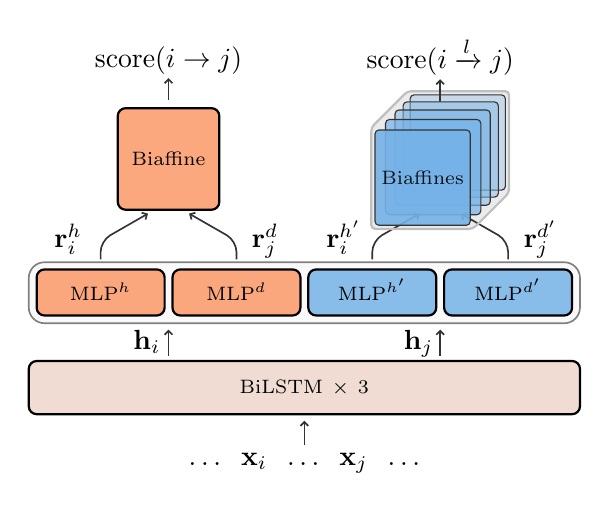
\begin{tikzpicture}[
        connect/.style={
                rounded corners=4pt,
                semithick,
                draw=black!80
            },
        arrow/.style={
                % >=latex,
                arrows = {-Straight Barb[length=0.5mm]},
                shorten >= 2pt,
                shorten <= 1.5pt,
                thin
            },
        inner arrow/.style={
                arrows = {-Straight Barb[length=0.4mm]},
                shorten >= 2pt,
                shorten <= 2pt,
                thin,
                draw=black!50
            },
        input/.style={
                rectangle,
                rounded corners=1mm,
                thin,
                dashed,
                draw=none,
                minimum width=3.5cm,
                minimum height=0.6cm,
            },
        share/.style={
                minimum height=0.5cm,
                fill={rgb,255:red,230; green,197; blue,180},
                % fill={rgb,255:red,240; green,245; blue,229},
                fill opacity=0.6,
                text opacity=1.0,
                draw=black,
                % thick,
                rounded corners=2mm,
            },
        task2/.style={
                minimum height=0.5cm,
                fill={rgb,255:red,251; green,153; blue,104},
                fill opacity=0.6,
                text opacity=1.0,
                draw=black,
                rounded corners=2mm,
            },
        label/.style={
                inner sep=0.5mm,
                fill=white,
                minimum height=0.5cm,
            },
        task1/.style={
                minimum height=0.5cm,
                fill={rgb,255:red,117; green,178; blue,231},
                draw=black,
                rounded corners=2mm
            },
        inner lstm/.style={
                fill=white,
                rectangle,
                rounded corners=1mm,
                semithick,
                % thin,
                draw=black!50,
                fill opacity=0.8
            },
        cell/.style={
                inner sep=2mm,
                rectangle,
                rounded corners=1mm,
                semithick,
                draw=black!50,
            },
        ocell/.style={
                solid,
                minimum height=0.5cm,
                rectangle,
                rounded corners=1mm,
                thick
            },
        dep arrow/.style={
        arrows = {-Latex[round,open,length=8pt,width=6pt]},
        shorten >= 2pt,
        shorten <= 1.5pt,
        thick
        }
        ]
        \centering
        \node [input, inner sep=1pt] [minimum width=4.8cm] (input) at (0, 0) {$\ldots\;\; \mathbf{x}_i \;\;\ldots\;\; \mathbf{x}_j \;\;\ldots$};
        % Concat
        \node [inner sep=0] (EmbedCat) at ($(input.north)$) {};
    
        %\scriptsize BiLSTM
        \node [share, ocell] [minimum width=7cm, minimum height=0.675cm, anchor=south] (lstm) at ($(input.north) + (0, 0.3cm)$) {\scriptsize $\mathrm{BiLSTM}\, \times \, 3$};
    

        \draw [arrow, connect] ($(EmbedCat.north) + (0cm, -0.15cm)$) -- ($(lstm.south) + (0cm, 0)$);


        % fisrt two mlps
        \node [share, fill={rgb,255:red,245; green,245; blue,245}, semithick, draw=gray] [minimum width=7cm, minimum height=0.775cm, anchor=south] (share-mlp) at ($(lstm.north) + (0cm, 0.455cm)$) {};
        

        \node [task2, ocell] [minimum width=1.625cm, minimum height=0.585cm, anchor=south west, fill opacity=0.85] (mlp-1-1-f) at ($(lstm.north west) + (0.1cm, 0.55cm)$) {};
        \node [task2, ocell] [minimum width=1.625cm, minimum height=0.585cm, anchor=south west, fill opacity=0.85] (mlp-1-1-b) at ($(lstm.north west) + (1.825cm, 0.55cm)$) {};
        \node [anchor=base] at  ($(mlp-1-1-f.south) + (0, 0.2cm)$)  {\scriptsize $\mathrm{MLP}^{h}$};
        \node [anchor=base] at  ($(mlp-1-1-b.south) + (0, 0.2cm)$)  {\scriptsize $\mathrm{MLP}^{d}$};
    
        \node [task2, ocell, fill=none, draw=none] [minimum width=1.75cm, minimum height=0.40cm, anchor=south east, fill opacity=0.5, draw opacity=0.6] (mlp-1-2-b) at ($(mlp-1-1-b.north east) + (0, 0.5cm)$) {};
    
        \node [task2, ocell, anchor=south, fill opacity=0.85, minimum height=1.29cm, minimum width=1.29cm, align=center] (arc-biaffine) at ($(mlp-1-1-f.north)!0.5!(mlp-1-1-b.north) + (0, 0.73cm)$) {\scriptsize $\mathrm{Biaffine}$};
    
        \draw [arrow, connect] ($(mlp-1-1-b.north) + (0, 0.06cm)$) -- ($(mlp-1-1-b.north) + (0, 0.35cm)$) -- ($(arc-biaffine.south) + (0.2, 0)$);
        \draw [arrow, connect] ($(mlp-1-1-f.north) + (0, 0.06cm)$) -- ($(mlp-1-1-f.north) + (0, 0.35cm)$) -- ($(arc-biaffine.south) + (-0.2, 0)$);
    
        % second two mlps
        \node [task1, ocell] [minimum width=1.625cm, minimum height=0.585cm, anchor=south east, fill opacity=0.85] (mlp-2-1-f) at ($(lstm.north east) + (-1.825cm, 0.55cm)$) {};
        \node [task1, ocell] [minimum width=1.625cm, minimum height=0.585cm, anchor=south east, fill opacity=0.85] (mlp-2-1-b) at ($(lstm.north east) + (-0.1cm, 0.55cm)$) {};
        \node [anchor=base] at  ($(mlp-2-1-f.south) + (0, 0.2cm)$)  {\scriptsize $\mathrm{MLP}^{h'}$};
        \node [anchor=base] at  ($(mlp-2-1-b.south) + (0, 0.2cm)$)  {\scriptsize $\mathrm{MLP}^{d'}$};
    
        \node [anchor=south, minimum height=1.29cm, minimum width=1.29cm, draw=none] (label-biaffine-invis) at ($(mlp-2-1-f.north)!0.5!(mlp-2-1-b.north) + (0, 0.73)$) {};
    
        \filldraw[task1, ocell, fill={rgb,255:red,235; green,235; blue,235}, draw=none, rounded corners=0.5mm] ($(mlp-2-1-f.north)!0.5!(mlp-2-1-b.north) + (-0.875, 0.5)$) -- ($(mlp-2-1-f.north)!0.5!(mlp-2-1-b.north) + (0.415, 0.5)$) -- ($(mlp-2-1-f.north)!0.5!(mlp-2-1-b.north) + (0.875, 0.96)$) -- ($(mlp-2-1-f.north)!0.5!(mlp-2-1-b.north) + (0.875, 2.25)$) -- ($(mlp-2-1-f.north)!0.5!(mlp-2-1-b.north) + (-0.415, 2.25)$) -- ($(mlp-2-1-f.north)!0.5!(mlp-2-1-b.north) + (-0.875, 1.79)$) -- cycle;
    
        \draw [arrow, connect] ($(mlp-2-1-b.north) + (0, 0.06cm)$) -- ($(mlp-2-1-b.north) + (0, 0.35cm)$) -- ($(label-biaffine-invis.south) + (0.2, 0)$);
        \draw [arrow, connect] ($(mlp-2-1-f.north) + (0, 0.06cm)$) -- ($(mlp-2-1-f.north) + (0, 0.35cm)$) -- ($(label-biaffine-invis.south) + (-0.2, 0)$);
    
        \filldraw[task1, ocell, fill=none, draw=lightgray, rounded corners=0.5mm] ($(mlp-2-1-f.north)!0.5!(mlp-2-1-b.north) + (-0.875, 0.5)$) -- ($(mlp-2-1-f.north)!0.5!(mlp-2-1-b.north) + (0.415, 0.5)$) -- ($(mlp-2-1-f.north)!0.5!(mlp-2-1-b.north) + (0.875, 0.96)$) -- ($(mlp-2-1-f.north)!0.5!(mlp-2-1-b.north) + (0.875, 2.25)$) -- ($(mlp-2-1-f.north)!0.5!(mlp-2-1-b.north) + (-0.415, 2.25)$) -- ($(mlp-2-1-f.north)!0.5!(mlp-2-1-b.north) + (-0.875, 1.79)$) -- cycle;
    
        \node [anchor=south west, minimum height=1.29cm, minimum width=1.29cm, draw=none] (label-biaffine-f) at ($(mlp-2-1-f.north)!0.5!(mlp-2-1-b.north) + (-0.875, 0.5)$) {};

        \node [anchor=north east, minimum height=1.29cm, minimum width=1.29cm, draw=none] (label-biaffine-b) at ($(mlp-2-1-f.north)!0.5!(mlp-2-1-b.north) + (0.875, 2.25)$) {};  

        \node [fill={rgb,255:red,117; green,178; blue,231}, fill opacity=0.3, minimum height=1.21cm, minimum width=1.21cm, draw=black!80, rounded corners=0.5mm, align=center, inner sep=0.1mm] at ($(label-biaffine-f)!1.0!(label-biaffine-b)$) {};
    
        \node [fill={rgb,255:red,117; green,178; blue,231}, fill opacity=0.4, minimum height=1.21cm, minimum width=1.21cm, draw=black!80, rounded corners=0.5mm, align=center, inner sep=0.1mm] at ($(label-biaffine-f)!0.8!(label-biaffine-b)$) {};
    
        \node [fill={rgb,255:red,117; green,178; blue,231}, fill opacity=0.5, minimum height=1.21cm, minimum width=1.21cm, draw=black!80, rounded corners=0.5mm, align=center, inner sep=0.1mm] at ($(label-biaffine-f)!0.57!(label-biaffine-b)$) {};

        \node [fill={rgb,255:red,117; green,178; blue,231}, fill opacity=0.7, minimum height=1.21cm, minimum width=1.21cm, draw=black!80, rounded corners=0.5mm, align=center, inner sep=0.1mm] at ($(label-biaffine-f)!0.3!(label-biaffine-b)$) {};
        
        \node [fill={rgb,255:red,117; green,178; blue,231}, fill opacity=0.9, minimum height=1.21cm, minimum width=1.21cm, draw=black!80, rounded corners=0.5mm, align=center, inner sep=0.1mm] at ($(label-biaffine-f)!0.0!(label-biaffine-b)$) {\scriptsize $\mathrm{Biaffines}$};
    
        %  LSTM -> MLP
        \draw [arrow, connect, rounded corners=1.2pt, shorten >= 2pt] ($(lstm.north) + (-1.725cm, 0)$) -- ($(share-mlp.south) + (-1.725cm, 0)$);
        \draw [arrow, connect, rounded corners=1.2pt, shorten >= 2pt] ($(lstm.north) + (1.725cm, 0)$) -- ($(share-mlp.south) + (1.725cm, 0)$);
        \node[anchor=base] at ($(share-mlp.south) + (-2cm,-0.32cm) $) {$\mathbf{h}_{i}$};
        \node[anchor=base] at ($(share-mlp.south) + (1.45cm,-0.32cm) $) {$\mathbf{h}_{j}$};
    
    
        \node[anchor=base] at ($(share-mlp.north) + (-3.0cm,0.18cm) $) {$\mathbf{r}_{i}^{h}$};
        \node[anchor=base] at ($(share-mlp.north) + (-0.5cm,0.18cm) $) {$\mathbf{r}_{j}^{d}$};
        \node[anchor=base] at ($(share-mlp.north) + (0.5cm,0.18cm) $) {$\mathbf{r}_{i}^{h'}$};
        \node[anchor=base] at ($(share-mlp.north) + (3.0cm,0.18cm) $) {$\mathbf{r}_{j}^{d'}$};
    
    
        \node[anchor=base] at ($(arc-biaffine.north) + (0cm,0.5cm) $) (arc-biaffine-label) {$\mathrm{score}(i \rightarrow j)$};
        \node[anchor=base] at ($(label-biaffine-invis.north) + (0,0.5cm) $) (label-biaffine-label) {$\mathrm{score}(i \xrightarrow{l} j)$};
    
    
        \draw [arrow, connect, rounded corners=1.2pt, shorten >= 2pt] ($(arc-biaffine-label.south) + (0, -0.25cm) $) -- ($(arc-biaffine-label.south) + (0, 0.15cm) $);
        \draw [arrow, connect, rounded corners=1.2pt, shorten >= 2pt, line cap=round] ($(label-biaffine-label.south) + (0, -0.25cm) $) -- ($(label-biaffine-label.south) + (0, 0.15cm) $);
    
    \end{tikzpicture}
    
    \caption{
      The basic architecture of Biaffine Parser. 
    }
    \label{fig:biaffine-parser}
\end{figure}
We adopt the SuPar implementation released by  \citet{zhang-etal-2020-dep}.\footnote{\url{https://github.com/yzhangcs/parser}}  
As a graph-based parser, Biaffine parser casts a tree parsing task as searching for a maximum-scoring tree from a fully-connected graph, with nodes corresponding to characters in our case. As shown in Figure \ref{fig:biaffine-parser}, it adopts standard encoder-decoder architecture, consisting of the following components.  
%Biaffine parser is a graph-based dependency parser which employs a deep biaffine scoring architecture to compute the score of each dependency and aims to find the highest-scoring dependency tree.
%\subsection{Model Architecture}
% The model architecture is shown in Figure xxx, consisting of following four components. 
% it consists of three major layers. 

\textbf{Input layer.} 
Given an input sequence, 
%consisting of $n$  $c_0c_1...c_n$, where $c_i$ is the $i$-th character and $c_0$ is a pseudo character used as tree root. 
each item is represented as a dense vector $\mathbf{x}_i$. 
For word-internal structure parsing, an item corresponds to a character, and we use char embedding. 
%the char representation output by BERT. 
%using the character embeddings $\mathbf{emb}^{c}$:
\begin{equation}
\mathbf{x}_i = \mathbf{emb}(c_i) 
% \oplus \mathbf{emb}^{bc}(c_{i-1}c_i)
\end{equation}

\textbf{BiLSTM encoder.} 
Then, a three-layer BiLSTM is applied to obtain  context-aware representations. 
We denote the hidden vector of the top-layer BiLSTM for  the i-th position as $\mathbf{h}_i$.

\textbf{Biaffine scorer.} %MLP feature abstraction.} 
Two separate MLPs are applied to each $\mathbf{h}_i$, resulting in 
%fed into two separate MLPs to 
%producing 
two lower-dimensional vectors $ \mathbf{r}_{i}^{h}$ (as head) and $\mathbf{r}_{i}^{d}$ (as dependent).
Then the score of a dependency $i \rightarrow j$ is obtained via a biaffine attention over $\mathbf{r}_{i}^{h}$ and $\mathbf{r}_{j}^{d}$. 
%To save space, we omit the 
Scoring of labeled dependencies such as $i \xrightarrow{l} j$ is analogous. 

%, representing  as a head and a dependent respectively. 
% \begin{equation}
%     \mathbf{r}_{i}^{h} = {\textup{MLP}}^{h} \left(\mathbf{h}_i \right) ;
%     \mathbf{r}_{i}^{d} = {\textup{MLP}}^{d} \left(\mathbf{h}_i \right)
% \end{equation} 
%\textbf{Biaffine classifier.} 
%The biaffine classifier computes 
% \begin{equation} \label{eq:biaffine}
%  \texttt{s}(i \leftarrow j) =  \left[
%  \begin{array}{c}
%     \mathbf{r}_{i}^{d}    \\
%       1 
%  \end{array} 
%  \right]^\mathrm{T}  \mathbf{W}^{biaffine}  \mathbf{r}_{j}^{h} 
% \end{equation} 
% where ${\mathbf{W}^{biaffine}}$ is a biaffine parameter.

% Analogously, the parser uses extra MLPs and a biaffine attention to compute scores for dependency labels. Please refer to \citet{dozat2016deep} for details.

\textbf{Decoder. }
%During decoding, the biaffine parser treats unlabeled dependency tree searching and dependency labeling as two cascaded tasks.
% First, with the scores of all dependencies, the score of a unlabeled dependency tree $\bm{y}$ is:
% \begin{equation}
% \begin{split}
% \texttt{s}(\bm{y})= \sum_{{{i \leftarrow j} \in \bm{y}}}\texttt{s}(i \leftarrow j)
% \end{split}
% \end{equation}
With the scores of all dependencies, 
we adopt the first-order algorithm of \citet{Eisner2000} % for projective decoding 
to find the optimal unlabeled dependency tree, and then independently decide the highest-scoring label for each arc. 
%$\bm{y}^{*}$ with the highest score from all the possible trees.
%Then, the biaffine parser finds the highest-scoring label for each dependency of the optimal tree $\bm{y}^{*}$.


\textbf{Training loss.} %with Local Char-wise Loss}
During training, the parser computes two independent cross-entropy losses for each position, i.e., maximizing the probability of its correct head and
%, and maximizing the probability of 
the correct label between them. 
%$c_j$ and the corresponding correct dependency label $l$ for each character $c_i$ independently.
% \begin{equation}
% \begin{split}
%  \texttt{loss}(i \xleftarrow{l} j) = &-\log{ 
% \frac{e^{\texttt{s}(i \leftarrow j)}}
% {\sum\limits_{0 \le k \le n, k \neq i}e^{\texttt{s}(i \leftarrow k)}} 
% }\\
% & -\log{ 
% \frac{e^{\texttt{s}(i \xleftarrow{l} j)}}
% {\sum\limits_{l' \in \mathcal{L}}e^{\texttt{s}(i \xleftarrow{l'} k)}} 
% }
% \end{split}
% \end{equation}
% where $\texttt{s}(i \xleftarrow{l} j)$ is the score of labeling the dependency $i \leftarrow j$ as $l$. $\mathcal{L}$ is the whole dependency label set.





%\subsection{Experiments and results}
\subsection{Settings}

\textbf{Data.} We randomly split all words in WIST into three parts, 2,500/5,000 as development/test data and remaining as training data. 
%We conduct experiments on our manually annotated char-level syntactic treebank, which consists of 25,531, 2,504, and 5,013 words in training, development, and test sets respectively.

\textbf{Hyperparameters.} 
We set the dimension of char embeddings to 100. 
We obtain pre-trained character embeddings by training  word2vec on Chinese Gigaword Third Edition.
%We adopt the 100 dimension character embeddings of %\citet{liying-2019} 
%pretrained with word2vec model on Chinese Gigaword.
In order to see effect of contextualized character representations, we apply BERT \cite{devlin-2019-bert} \footnote{BERT-base-Chinese:\url{https://github.com/google-research/bert}} to each word as a char sequence. The output vectors of the top four layers are concatenated and reduced into a dimension of 100 via an MLP. 
For other hyper-parameters, we keep the default configuration in SuPar.
%We adopt most of the parameter settings in the open source parser \cite{dozat2016deep}. 
%Each model is trained for at most 1000 iterations. We stop training when the peak performance on the development data does not increase in 100 consecutive iterations. 


%The dimension of char embedding is set to 50. 
\textbf{Evaluation metrics.} 
We adopt the standard unlabeled and labeled attachment score (UAS/LAS), i.e., the percent of characters that receives the correct head (and label). 
%The unlabeled and labeled complete matches (UCM/LCM) is the percent of words having correct whole trees.
The complete match (CM) is the percent of words having correct whole trees.

\setlength{\tabcolsep}{3.6pt}
\begin{table}[tb]
%\setlength{\leftskip}{-25pt}
\begin{center}
% \begin{small}
\begin{tabular}{l  rr rrr }
\toprule
\multirow{2}{*}{} 
& \multicolumn{2}{c}{Dev }
& \multicolumn{3}{c}{Test} \\
\cmidrule(lr){2-3} \cmidrule(lr){4-6}
% \cline{2-6}
& UAS & LAS & UAS & LAS & CM\\
\hline
Random & 81.18 & 76.15  & 80.63 & 75.58 & 65.13 \\[2pt]
%\hline
\multirow{2}*{Pretrained}
 & 82.42 & 77.30 & 81.64 & 76.98  & 67.09 \\
 & +1.24 & +1.15 & +1.01 & +1.40 & +1.96\\[2pt]
%\hline
\multirow{2}*{BERT} 
 & 88.27 & 85.18 & 88.33 & 84.98 &77.72\\
 & +5.85 & +7.88 & +6.69 & +8.00 & +10.63\\
\bottomrule
\end{tabular}
% \end{small}
\caption{Results of word-internal structure parsing using different character representations.} 
\label{iwdp-result}
\end{center}
\end{table}


\subsection{Results}

Table \ref{iwdp-result} shows the main results  %word-internal structure parsing 
under different char representations.  
% It turns out that word-internal structure parsing is not a piece of cake.
% The best model integrated BERT representations\footnote{The BERT in the experiment is ``bert-base-chinese'' released by \citet{peters2018deep}.}, which outperforms those without BERT  by over 10 in LAS, merely achieves a LAS of 84.98 and a LCM of 77.72.
% Pretrained char embeddings are also helpful to the word-internal structure parsing.
% But it only brings improvement by 1.40 in LAS and 1.96 in LCM, compared with the model using randomly initialized char embeddings.
It is obvious that using randomly initialized char embeddings, the parser can only reach about 76 in LAS. This shows that parsing word-internal structure is very challenging without using extra resources. 
When we pretrain char embeddings on large-scale labeled data, the performance can be consistently improved by over 1 point in both UAS/LAS, and nearly 2 points in CM. 
Finally, employing the contextualized character representations dramatically improves performance further by about 6/8/10 points in UAS/LAS/CM. 

However, even with BERT, model performance still lags behind averaged human performance (90.9 in LAS) by large margin.
Our experienced annotators can even reach more than 94. 
Our experience in manual annotation points out two possible directions to enhance the model: 1) making use of sentence-level contextual information; 2) leveraging the meanings in dictionaries, usually in the form of explanation or example sentences. 
We leave them for future exploration. 

%without  using pretrained char embeddings brings substantial improvement by 1.40 in LAS and 1.96 in LCM on test. 

%Integrating with BERT representations\footnote{The BERT in the experiment is ``bert-base-chinese'' released by \citet{peters2018deep}.} can further boost the model performance by a very large margin, outperforming those without BERT by over 8 in LAS and over 10 in LCM on test. 

\textbf{Analysis on label-wise accuracy.}
% Using BERT representations can further improve the parser by a very large margin.
%\begin{figure}[tb]
  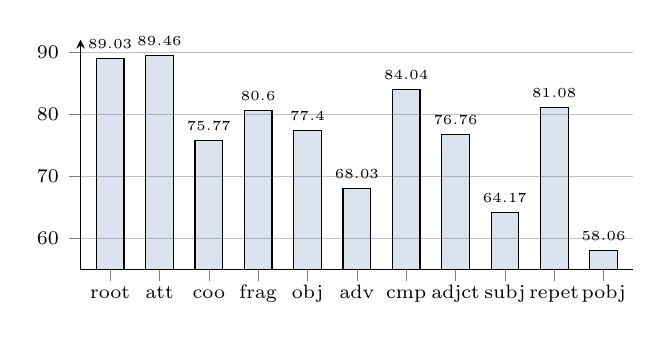
\begin{tikzpicture}
    \begin{axis} [
        width=8.6cm, height=4.5cm,
        ybar,
        axis y line=left,
        axis x line=left,
        x axis line style={-},
        ymajorgrids=true,
        enlarge x limits=0.06,
        tick align=outside,
        ymin=55, ymax=92,
        symbolic x coords={
            root, att, coo, frag, obj, adv, cmp, adjct, subj, repet, pobj
        },
        xtick=data,
        nodes near coords=\pgfmathprintnumber\pgfplotspointmeta,
        xticklabel shift=6,
        x tick label style={anchor=base, font=\scriptsize},
        y tick label style={font=\scriptsize},
    ]
    \addplot [
        draw=black,
        fill opacity=0.2, 
        text opacity=1,
        font=\tiny, 
        fill={rgb,255:red,76; green,114; blue,176}] coordinates {
        (root, 89.03)
        (att, 89.46)
        (coo, 75.77)
        (frag, 80.6)
        (obj, 77.4)
        (adv, 68.03)
        (cmp, 84.04)
        (adjct, 76.76)
        (subj, 64.17)
        (repet, 81.08)
        (pobj, 58.06)
    };
  \end{axis}
\end{tikzpicture}

\caption{
  Accuracy on different dependency labels.
}
\label{fig:model-acc}
\end{figure}

The second major row in Table \ref{table:label distribution} reports accuracy regarding different labels for the model with BERT. 
The model achieves the highest accuracy on ``att'' and ``root'', possibly because the two labels take very large proportion in the data for sufficient model training. 
%One direct reason is that these two labels accounts for the largest proportion of all labels, and thus the model can be trained sufficiently. 
% , indicating that it is relatively easy for the model to recognize the head character for each word.
%Moreover, it is easy to recognize ``att'' since the word with ``att'' label usually has a typical modifier-noun structure, which is very common in Chinese words and usually frequently occurs in the training data. 
%For ``root'', it represents the most important head character that conveys the main meaning of each word, such head characters are also high-frequency characters and thus can be distinguished with other unimportant characters. 
By contrast, ``pobj'' and ``subj'' have the lowest accuracy, and are difficult for models as well as discussed in Section \ref{sec:data-annotation}. 
%performance, achieving only ``58.1'' in accuracy.
%By carefully checking the predicted results, we find that the model usually confuses ``pobj'' with ``obj''. In fact, these two labels are quite similar in syntax. The proportion of ``obj'' is much larger than ``pobj'' (5.4 vs. 0.2). The sample imbalance problem causes the model to lean to label ``pobj'' as ``obj''.
This leads to 
another observation that model accuracy is roughly correlated with annotation accuracy, implying the difficulties for human and model are usually consistent. 
% However, it is not easy for the model to correctly recognize ``subj'' and ``pobj'', achieving only ``64.2'' and ``58.1'' in accuracy respectively. By carefully checking the predicted results, we find that the model usually confuses ``subj'' with  ``adv'' and confuses ``obj'' with ``pobj''.

% the sample imbalance problem causes the model to lean to label “激动(excite)” as an adjective



% as illustrated in Table \ref{table:label distribution}, and thus the model can be trained sufficiently. 

% coo和adv容易混淆

% and ``att''

% the proportion of these 

% account for a relatively large proportion in all the labels


% whereas the lowest accuracy on ``subj'' and ``pobj'', which is consistent with the manual annotation accuracy.



% root和att准确率高是因为:1.root标签属于核心字,是一个词中最为核心的部分,往往承载着一个词的主要意思,因此比较容易找出。att标签准确率高我觉得是因为att标签数量多,如果核心字是名词性字,那么它前面的字很有可能是att,容易识别,特征明显。subj难识别是因为,subj标签容易被误标注成adv标签,对于是主语还是修饰关系,有时候难以理解,pobj标签错误率高更大原因是因为难以分辨到底是obj还是pobj,比如在这个字,一般认知下会觉得是介词,但是其实在单个字中,在通常作为动词,形成obj



%\input{content/encode-iwdp-for-dependency}
% \section{Sentence-level syntactic Parsing with Structure-aware Word Representation}

\section{Utilizing Word-internal Structure}

This section presents a preliminary study on utilizing word-internal structure, aiming to address the third question: is modeling word-internal structures beneficial for word representation learning? 
% We conduct our study on sentence-level dependency parsing to make investigation on whether integrating structure-aware word representation can be beneficial. 
% 【用解释为啥在句法分析上做实验吗?】

We use sentence-level dependency parsing as the focusing task \cite{KublerDEP09}, mainly considering resemblance in tree structure representation and close relatedness between the two tasks. 
% We also 
Given an input sentence $w_0w_1...w_m$, 
%where $w_i$ is  the $i$-th word and $w_0$ is a pseudo word for sentence start, sentence-level dependency 
the goal of dependency parsing is to find an optimal dependency tree for the sentence. 
%the head word $w_j$ for each word $w_i$ and the dependency relation label between $w_i$ and $w_j$.
%Similar to the word-internal structure parsing as described in Section \ref{char-pasrsing}, w
Again, we adopt SuPar \cite{zhang-etal-2020-dep} for implementation of Biaffine parser \cite{dozat2016deep} % and the implementation of  
as our basic parser. 
%for sentence-level dependency parsing. 


\subsection{Methods}

The basic parser applys a BiLSTM over character sequence to obtain word representation. 
In this part, we propose two  simple alternative methods to encode internal structure shown in Figure \ref{fig:example}-(c).

\textbf{Basic CharLSTM method.} For each word, the basic Biaffine parser uses the concatenation of word embeddings and CharLSTM outputs to represent each word in the input layer:
\begin{equation}\label{eq:charlstm-eq}
\begin{split}
& \mathbf{x}_i = \mathbf{emb}(w_i) 
 \oplus \textup{CharLSTM}(w_i) \\
& \textup{CharLSTM}(w_i) \leftarrow \textup{BiLSTM}(...,\mathbf{z}_{k},...) \\
& \mathbf{z}_{k} = \mathbf{emb}(c_{i,k}) 
\end{split}
\end{equation}
where $c_{i,k}$ is the k-th character of $w_i$. The final word representation from $\textup{CharLSTM}(w_i)$ 
is obtained by concatenating two last-timestamp hidden output vectors of a one-layer BiLSTM. 
%The other parts of the model architecture for the sentence-level dependency parsing remain consistent with the word-internal structure parsing as described in section \ref{char-pasrsing}.

% To exploit the syntactic word-internal information for sentence-level parsing, we investigate and compare two methods to encode the syntactic word-internal structures.
% Each method produces a representation considering the word-internal structure of the concerned word $w_i$, which is denoted as $\mathbf{r}_i^{syn}$.
% We treat the syntactic structure-aware representation $\mathbf{r}_i^{syn}$ of word $w_i$ as extra features and concatenate it with the original input $\mathbf{x}_i^w$.
% We introduce the two methods in detail in the following subsections.


\textbf{LabelCharLSTM Method.} 
% 谁的方法说明,用label embedding就很有效果了。
% \textbf{Encoding with sequence model.}
%Previous work on syntax-aware semantic role labeling shows it is simple and effective to %of using syntactic trees is to 
%feed syntactic label embeddings as extra inputs into encoders \cite{XXXX}. 
Considering that the word is usually very short and a bare label itself provides rich syntax information,  
we propose a straightforward extension to CharLSTM, named as LabelCharLSTM, via minor modification.%  to Equation \ref{eq:charlstm-eq}.
\begin{equation}\label{eq:labelcharlstm-eq}
\begin{split}
& \mathbf{z}_{k} = \mathbf{emb}(c_{i,k}) \oplus \mathbf{emb}(l_{i,k})
\end{split}
\end{equation}
where $l_{i,k}$ represents the label between $c_{i,k}$ and its head in the word-internal structure. 
%concatenating char with label embedding 
% Apart from the novel graph neural network, we also utilize CharLSTM, without changing the major network structure of baseline model, to integrate structure-aware word representations.
% 除了使用新颖的图神经网络之外,我们还给出另外一个十分直接的引入字结构表示信息的方法,which 我们不需要引入别的神经网络结构。
% 师姐我说我们用charLSTM编码label的初衷是,
% In syntactic parsing task, one of the most important role of the CharLSTM is to explore the part-of-speech clues of a word from characters it contained.
% For Chinese language, 【可以说,中心词以及非中心字的语法角色隐含了词性信息吗? 比如``枣红''的中心字是``红'',而``红枣''的中心字是``枣''】.
%As depicted in Table \ref{table:summary-different-num-word}, about $92.1\%$ words in the dataset are one-character words or two-character words.
%Their word-internal skeleton trees are simple, but the word-internal dependency labels still can provide clues. We encode such dependency label information by employing a BiLSTM.
% by pointing out center-character and illustrating the function of non-center-characters.
% So, we omit the arcs of the word-internal structures.
% , and feed each character together with its relation labels into the CharLSTM.
% That is, for now, the input of CharLSTM in Equation \ref{baseline-input} is $w_i$ and $l_{u,v}$, the label of dependency $u \leftarrow v$. 【这里的的公式还有些奇怪,得再改一下】
% 在依存解析中,charLSTM的一个很重要的任务是去从组成词的字中发掘POS信息。我们发现基于这个出发点 词内部的每个字的label要比字符间的依存弧更为重要,因为它可以指出哪个字为词语的中心字并标明不同字在词语中所承担的角色。因此我们为了使得模型更加简单而忽略arc。
%Formally, we concatenate the character embedding with the dependency label embedding, and then go through a single-layer BiLSTM:
% \begin{equation}
%     % [\overrightarrow{\mathbf{h}}_{u}, \overleftarrow{\mathbf{h}}_{u} ] =\textup{BiLSTM}(\mathbf{emb}^{c}(c_u) \oplus \mathbf{emb}^{l}(l_{u,v}))
%     {\mathbf{h}}_{u} =\textup{BiLSTM}(\mathbf{emb}^{c}(c_u) \oplus \mathbf{emb}^{l}(l_{u,v}))
% \end{equation}
% Here, $\mathbf{emb}^{l}(l_{u,v})$ is the label embedding for dependency $u \leftarrow v$.
% The pooling operation is performed on the top-layer ouputs of BiLSTM to obtain $\mathbf{r}_i^{syn}$, which is the same as Equation \ref{pooling}. 



% \subsection{Representation with GCN}
% We employ two different models to encode syntactic word-internal structures explicitly.
\textbf{LabelGCN method.} 
%缩写应该在intro提到才对,到时候确认
% \textbf{Encoding with graph model.} 
Previous work show that GCN is very effective in encoding
%The graph convolutional network (GCN) \cite{kipf2016semi} is designed for modeling graph structures, and can be naturally used for exploiting
syntactic trees \cite{marcheggiani-titov-2017,zhang-etal-2018}. 
%In this work, we employ GCN to encode the word-internal structure of Chinese words. 
We follow the implementation of \citet{zhang-etal-2018} and use a two-layer GCN as a more sophisticated way. % to encode word-internal structure. 
In order to utilize labels, we extend vanilla GCN to have the same input with 
% Formally, given a internal structure of a word with $t$ nodes (each node is a character), we use an $t \times t$ adjacency matrix $\mathbf{{A}}$ to represent such structure, where $A_{uv}=1$ if there is a dependency arc between the $u$-th node $c_u$ and the $v$-th node $c_v$. Following \citet{marcheggiani-titov-2017}, we also set the diagonal elements of $\mathbf{{A}}$ to $1$ to add a self-loop for each node.
% The input of GCN is the same with
LabelCharLSTM, i.e., $\mathbf{z}_{k}$.
We obtain the final word representation by performing average pooling over the output vectors of the top-layer GCN.  
% The representation vector $\mathbf{h}_u^m$ of the node $c_u$ at the $m$-th layer of GCN is computed based on its one-hop neighbours and itself, which is defined as:
% \begin{equation}\label{GCN}
%     \begin{split}
%     \mathbf{h}_{u}^{m}&=\rho\Bigg( \sum_{v=1}^{n}{\mathbf{{A}}_{uv}}\mathbf{W}^{m}\mathbf{h}_v^{m-1} + \mathbf{b}^{m}\Bigg)
%     \end{split}
% \end{equation}
% where $\mathbf{W}^{m}$ and $\mathbf{b}^{m}$ are model parameters. $\rho$ denotes an activation function. 
% $\mathbf{h}_u^0$ is the initial input representation to GCN, which is the concatenation of the character embedding and the dependency label embedding.
% \begin{equation}
%     \mathbf{h}_{u}^{0}=\textup{BiLSTM}(\mathbf{emb}^{c}(c_u) \oplus \mathbf{emb}^{l}(l_{u,v}))
% \end{equation}
% Here, $\mathbf{emb}^{l}(l_{u,v})$ is the label embedding for dependency $u \leftarrow v$.
% 【h0不用BiLSTM了,后面改】
% 【双向还没写,看实验结果】
% The final syntactic structure-aware representation $\mathbf{r}_i^{syn}$ for the word $w_i$ is obtained by performing an average pooling operation on the top-layer outputs of the GCN which contains $M$ layers in total.
% % Finally, an average pooling operation is performed on the top-layer GCN outputs to obtain the syntactic structure-aware representation $\mathbf{r}_i^{syn}$ for the word $w_i$.
% \begin{equation}
% \mathbf{r}^{syn}_{i} =
% \textup{Pooling}(\{\mathbf{h}_u^M|1 \leq u \leq t\})
% \label{pooling}
% \end{equation}

%\subsection{Representation with BiLSTM}
% \textbf{Encoding with sequence model.}
Apart from the novel graph neural network, we also utilize CharLSTM, without changing the major network structure of baseline model, to integrate structure-aware word representations.
% 除了使用新颖的图神经网络之外,我们还给出另外一个十分直接的引入字结构表示信息的方法,which 我们不需要引入别的神经网络结构。
% 师姐我说我们用charLSTM编码label的初衷是,
% In syntactic parsing task, one of the most important role of the CharLSTM is to explore the part-of-speech clues of a word from characters it contained.
% For Chinese language, 【可以说,中心词以及非中心字的语法角色隐含了词性信息吗? 比如``枣红''的中心字是``红'',而``红枣''的中心字是``枣''】.
As depicted in Table \ref{table:summary-different-num-word}, about $92.1\%$ words in the dataset are one-character words or two-character words.
Their word-internal skeleton trees are simple, but the word-internal dependency labels still can provide clues. We encode such dependency label information by employing a BiLSTM.
% by pointing out center-character and illustrating the function of non-center-characters.
% So, we omit the arcs of the word-internal structures.
% , and feed each character together with its relation labels into the CharLSTM.
% That is, for now, the input of CharLSTM in Equation \ref{baseline-input} is $w_i$ and $l_{u,v}$, the label of dependency $u \leftarrow v$. 【这里的的公式还有些奇怪,得再改一下】
% 在依存解析中,charLSTM的一个很重要的任务是去从组成词的字中发掘POS信息。我们发现基于这个出发点 词内部的每个字的label要比字符间的依存弧更为重要,因为它可以指出哪个字为词语的中心字并标明不同字在词语中所承担的角色。因此我们为了使得模型更加简单而忽略arc。
Formally, we concatenate the character embedding with the dependency label embedding, and then go through a single-layer BiLSTM:
\begin{equation}
    % [\overrightarrow{\mathbf{h}}_{u}, \overleftarrow{\mathbf{h}}_{u} ] =\textup{BiLSTM}(\mathbf{emb}^{c}(c_u) \oplus \mathbf{emb}^{l}(l_{u,v}))
    {\mathbf{h}}_{u} =\textup{BiLSTM}(\mathbf{emb}^{c}(c_u) \oplus \mathbf{emb}^{l}(l_{u,v}))
\end{equation}
Here, $\mathbf{emb}^{l}(l_{u,v})$ is the label embedding for dependency $u \leftarrow v$.
The pooling operation is performed on the top-layer ouputs of BiLSTM to obtain $\mathbf{r}_i^{syn}$, which is the same as Equation \ref{pooling}. 
% The final syntactic structure-aware representation $\mathbf{r}_i^{syn}$ 
% The final representation $\mathbf{r}_i^{syn}$ is the concatenation of $\overrightarrow{\mathbf{h}}_{n}$, the forward hidden representation of the last word of the sentence, and $\overleftarrow{\mathbf{h}}_{0}$, the backward representation of the first word.
% The final representation $\mathbf{r}_i^{syn}$ is the top-layer BiLSTM outputs.





% In addition to directly encoding the syntactic word-internal tree structure with the graph model GCN, we also employ the sequence model BiLSTM to obtain the structure-aware word representation.

%\input{content/encode-iwdp-exp}


%\subsection{Experiments and results}
\subsection{Experiments}

\paragraph{Settings.} Following \citet{chen-manning-2014fast}, we conduct experiments on CTB5 with the same data split (16,091/803/1,910 sentences) and constituent-to-dependency conversion. 
%(CTB5) with dependencies obtained by the Penn2Malt tool \footnote{http://stp.lingfil.uu.se/∼nivre/research/Penn2Malt.html}. 
%Most of the hyper-parameter settings is adopted from \citet{dozat2016deep}, expect settings of CharLSTM.
Both char/label embeddings are randomly initialized and have the same dimension of 50. 
For the parsers using gold-standard POS tags, we randomly initialized the POS tagging embeddings and set the dimension to 50.
For other hyperparameters, we adopt the default configuration of SuPar, including the pre-trained word embeddings. 
%We adopt the de
%and hidden layer of CharSLTM are set to 50. 
% We also obtain pre-trained word embeddings by training word2vec on Chinese Gigaword V3.
%Third Edition 【todo 是否用缩写?】

For multi-char words without annotated internal structure, we use the automatic outputs from the trained parser with BERT in Section \ref{sec:WIS-parsing}, so that every word corresponds to a single structure.  
%实验部分要给出所有词的词内部结构怎么来的。预测。
%所有词的内部结构都是给定的,每个词给一个。

We use word-wise UAS/LAS/CM for evaluation, and punctuation is excluded in all metrics.
% We adopt the same data split as \citet{zhang-clark-2008} on CTB5 and the gold standard data split on CoNLL09.
% Then, we obtain dependencies from CTB5 by the Penn2Malt tool \footnote{http://stp.lingfil.uu.se/∼nivre/research/Penn2Malt.html} and find corresponding constituent trees from Chinese Penn Treebank 6.0 (CTB6) according to CoNLL09 data.
% For dependency parsing, we use unlabeled and labeled attachment score (UAS/LAS) as main metrics. 
% For constituent parsing, we use the standard constituent-level labeled precision, recall and F-score (P/R/F) as the evaluation metric.

\paragraph{Main results.}

Table \ref{table:results-dependency} shows the parsing performance. We can see that both LabelCharLSTM and LabelGCN substantially outperform the basic CharLSTM method. 
LabelGCN achieves the best performance on UAS and LAS, with a gain of 0.71 and 0.80 respectively. 

The fourth row reports performance of LabelGCN without using label embedding, leading to consistent accuracy drop, demonstrating the usefulness of rich labels, which is a key contribution of this work, despite the extra annotation effort. 
%Without encoding word-internal skeleton tree, the BiLSTM approach already achieves improvement of 0.37/0.47 in UAS/LAS.
%Integrating the arc information by using GCN can further improve parsing performance by 0.56/0.63 in UAS/LAS.

% \begin{table}[tb]
% \setlength{\tabcolsep}{6.5pt}
% \centering
% \begin{tabular}{lccccc}
%     \toprule
%     & \multicolumn{2}{c}{Dev} & \multicolumn{3}{c}{Test} \\
%     & UAS & LAS & UAS & LAS & CM \\[2pt]
%     \hline
%     \\[-8pt]
%     Baseline &87.03 &85.05 &87.31 &85.23 &30.73 \\
%     BiLSTM   &87.03 &\textbf{85.22} &87.68 &85.70 &31.68 \\
%     GCN      &\textbf{87.13} &85.19 &\textbf{87.87}  &\textbf{85.86} & \textbf{31.78} \\
%     GCN w/o label &86.87 &84.76 &87.55 &85.41 &31.36\\
%     GCN 波浪 &87.06 &85.05 &87.56 &85.47& 31.15  \\

%     \bottomrule
% \end{tabular}
%     \caption{Main results for dependency parsing.}
%     \label{table:results-dependency}
% \end{table}

% \begin{table}[tb]
% \setlength{\tabcolsep}{6.5pt}
% \centering
% \begin{tabular}{lccccc}
%     \toprule
% %    &  \multicolumn{3}{c}{Test} \\
%     &  UAS & LAS & CM \\
%     \hline
%     Basic CharLSTM &87.31 &85.23 &30.73 \\
%     LabelCharLSTM    &87.68 &85.70 &31.68 \\
%     \hline
%     LabelGCN       &\textbf{87.87}  &\textbf{85.86} & \textbf{31.78} \\
%     %\hline
%     $~~~~~$ w/o label  &87.55 &85.41 &31.36\\
% %    $~~~~~$ GCN 波浪  &87.56 &85.47& 31.15  \\
%     \bottomrule
% \end{tabular}
%     \caption{Parsing performance on CTB5-test.}
%     \label{table:results-dependency}
% \end{table}

\begin{table}[tb]
\setlength{\tabcolsep}{6.5pt}
\centering
\begin{tabular}{lccccc}
    \toprule
%    &  \multicolumn{3}{c}{Test} \\
    &  UAS & LAS & CM \\
    \hline
    Basic CharLSTM &88.31 &85.96 &32.04 \\
    LabelCharLSTM    &88.78 &86.51 &\textbf{33.19} \\
    \hline
    LabelGCN       &\textbf{89.02}  &\textbf{86.76} & 32.93 \\
    %\hline
    $~~~~~$ w/o label  &88.66 &86.28 &32.20\\
%    $~~~~~$ GCN 波浪  &87.56 &85.47& 31.15  \\
    \bottomrule
\end{tabular}
    \caption{Parsing performance on CTB5-test.}
    \label{table:results-dependency}
\end{table}

%\input{content/encode-iwdp-analysis}

% \begin{table}[tb]
% \setlength{\tabcolsep}{2pt}
% \centering
% \begin{tabular}{lcccccc}
%     \toprule
%     % \hline
%     & \multicolumn{3}{c}{Dev} & \multicolumn{3}{c}{Test} \\
%     & P & R & F & P & R & F \\[2pt]
%     \hline
%     \\[-8pt]
%     \multicolumn{7}{c}{CTB5} \\
%     Baseline &87.81 &86.36 &87.08 &87.42 &87.13 &87.27 \\
%     BiLSTM   &\textbf{88.12} &\textbf{86.82} &\textbf{87.46} &\textbf{87.80} &\textbf{87.45} &\textbf{87.62} \\
%     GCN      &87.73 &86.56 &87.14 &87.60 &87.33 &87.47\\
%     \hline
%     \\[-8pt]
%     \multicolumn{7}{c}{CoNLL09} \\
%     Baseline &88.35 &87.35 &87.84 &88.66 &87.58 &88.12 \\
%     BiLSTM &88.69 &87.76 &88.22 &88.85 &87.84 &88.34 \\
%     GCN & \\[2pt]

%     \bottomrule
% \end{tabular}
%     \caption{Main results for constituency parsing.}
%     \label{table:results-constituency}
% \end{table}


\begin{table}[!tb]
\setlength{\tabcolsep}{4.2pt}
\centering
\begin{tabular}{lrrrr}
    \toprule
    % \hline
   & all & $>2$ &$\le2$ & unk.  \\
    \hline
    % \\[-8pt]
    Basic CharLSTM &85.96& 86.42 &82.03 &81.73   \\[2pt]
    \multirow{2}*{LabelGCN} 
    &86.76& 87.10 &83.79 &84.30  \\
    & +0.80 &+0.68 & +1.76 &+2.57  \\
    \bottomrule
\end{tabular}
    \caption{Parsing LAS regarding to word frequency.}% of common/rare/unkown words.} % frequency}. % on CTB5-test.}
    \label{table:rare-word-las}
\end{table}

\paragraph{Analysis on rare words.} 
To gain more insights on how word-internal structure helps word representation learning, we divide the words in CTB5-test into several groups according to their frequency in CTB5-train, and report fine-grained accuracy in Table \ref{table:rare-word-las}. 
%To investigate whether our proposed word-internal structure can be beneficial to the parsing performance on rare words, we divide the words on test data into three categories according to their frequency on training data: words with frequency $\leq 2$, words with frequency $\leq 1$ and words out of the training data (OOV). Table \ref{table:rare-word-las} compares the parsing performance (LAS) of the baseline model and our model which encodes word-internal structure with GCN on the three categories. We also give the performance on the whole test data (overall) for reference. We observe that the improvements on the rare words and OOV words are consistently larger than that on the whole test data, which means the word-internal structures make more contribution to rare/OOV words than high-frequency words. The main reason is that the word-internal structures contain rich information on how multiple characters form a word, which is helpful for representing rare words via composing the meanings of characters.
We can see that the overall performance gain is mostly contributed by improvement over rare words with low frequency or totally unknown. 
This verifies that word-internal structures can help the model to better represent rare words. 


\begin{table}[t]
\setlength{\tabcolsep}{2.5pt}
\centering
\begin{tabular}{lrrrrr}
    \toprule
%    &  \multicolumn{3}{c}{Test} \\
    &  UAS & LAS \\
    \hline
    % \citet{chen-manning-2014fast} & 88.1 &85.7\\
%   \citet{ballesteros-2016-training}& 87.65&86.21&\\
%   \citet{kiperwasser-2016-simple} &87.6 &86.1&\\
%   \citet{acl16-Zhang-parsing} & 87.65 & 86.17 &\\
%   \citet{kuncoro-2016-distilling} &88.87 &87.30 \\
   \citet{ma-2017-neural} &89.05 &87.74 \\
   \citet{dozat2016deep} &89.30 &88.23 \\
%   Zheng (2017) & 89.42 &87.94\\
%   \citet{coling2018-seq2seqparsing} &88.78 &86.23\\
   \citet{acl18-ma-stackpointer} &\textbf{90.59}&\textbf{89.29}\\
    \hline
    Basic CharLSTM &91.11 &89.91  \\
    LabelCharLSTM    &\textbf{91.31} &90.15 \\
    LabelGCN       &\textbf{91.31}  &\textbf{90.16} \\
    %\hline
    % $~~~~~$ w/o label  &87.55 &85.41 &31.36\\
%    $~~~~~$ GCN 波浪  &87.56 &85.47& 31.15  \\
    \bottomrule
\end{tabular}
    \caption{Parsing performance with gold-standard POS tags on CTB5-test.}
    \label{table:results-dependency-goldpos}
\end{table}


\paragraph{Results with gold-standard POS tags.} As suggested by a reviewer, we train our parser with gold-standard POS tags by concatenating the original input (i.e., $\mathbf{x}_{i}$ in Equation \ref{eq:charlstm-eq}) with gold-standard POS tag embeddings, in order to compare with previous works. 
Table \ref{table:results-dependency-goldpos} shows the results. 
Compared with the Basic CharLSTM results in Table \ref{table:results-dependency}, using gold-standard POS tags as extra features for the Basic CharLSTM leads to substantial improvements by 2.80 and 3.95 in UAS and LAS respectively, and outperforms the previous works as presented in Table \ref{table:results-dependency-goldpos}, showing that the basic CharLSTM can be served as a strong baseline model.


% the Basic CharLSTM, LabelCharLSTM, and LabelGCN in Table \ref{table:results-dependency-goldpos} augment the input by concatenating the original input (i.e., $\mathbf{z}_{k}$) with the embeddings of gold-standard POS tags.

% When using gold-standard POS tags as extra features, the basic CharLSTM outperforms the previous works, showing that the basic CharLSTM can be served as a strong baseline model.

Compared with the Basic CharLSTM, utilizing word-internal structure with LabelCharLSTM or LabelGCN achieves consistently better performance by 0.24 and 0.25 respectively in LAS in the scenario of using gold-standard POS tags.
Besides the strong baseline, another reason that the improvement brings by the internal-word structure is slight when using gold-standard POS tags is that a part of linguistic information in the POS tags and the word-internal structures may be overlapping.

% less than that in the scenario of without using gold-standard POS tags


% Although the improvement is less than that in the scenario of without using gold-standard POS tags due to a part of overlapping information in POS tags and internal-word structures, we believe that the POS tags and internal-word structures can also provide complementary contributions to the parsing performance according to the slightly but consistently improvement. 
% We will explore





% \section{Experiment \& Analysis}
\label{sec:exp}
In this section, we first introduce the experimental set-up. Then, we report the performances of baselines and the proposed steep slope loss on ImageNet, followed by comprehensive analyses. 
% At last, we present comprehensive analyses to help better understand the efficacy of the proposed loss.

\noindent\textbf{Experimental Set-Up}.
We use ViT B/16 \cite{Dosovitskiy_ICLR_2021} and ResNet-50 \cite{He_CVPR_2016} as the classifiers, and the respective backbones are used as the oracles' backbones. We denote the combination of oracles and classifiers as \textlangle O, C\textrangle. There are four combinations in total, \ie \textlangle ViT, ViT\textrangle, \textlangle ViT, RSN\textrangle, \textlangle RSN, ViT\textrangle, and \textlangle RSN, RSN\textrangle, where RSN stands for ResNet.
In this work, we adopt three baselines, \ie the cross entropy loss \cite{Cox_JRSS_1972}, focal loss \cite{Lin_ICCV_2017}, and TCP confidence loss \cite{Corbiere_NIPS_2019}, for comparison purposes.

The experiment is conducted on ImageNet \cite{Deng_CVPR_2009}, which consists of 1.2 million labeled training images and 50000 labeled validation images. It has 1000 visual concepts. Similar to the learning scheme in \cite{Corbiere_NIPS_2019}, the oracle is trained with training samples and evaluated on the validation set. During the training process of the oracle, the classifier works in the evaluation mode so training the oracle would not affect the parameters of the classifier. Moreover, we conduct the analyses about how well the learned oracle generalizes to the images in the unseen domains. To this end, we apply the widely-used style transfer method \cite{Geirhos_ICLR_2019} and the functional adversarial attack method \cite{Laidlaw_NeurIPS_2019} to generate two variants of the validation set, \ie stylized validation set and adversarial validation set. \REVISION{Also, we adopt ImageNet-C \cite{Hendrycks_ICLR_2018} for evaluation, which is used for evaluating robustness to common corruptions.}
% Then, the oracle trained with regular training samples would be evaluated with the samples that are in the two unseen domains.

% To understand how the learned oracle work on unseen domains, the oracle is learned with training samples and is evaluated with three types of samples, the samples on the same domain as training samples and the samples on two unseen domains. We base our experiments on ImageNet \cite{Deng_CVPR_2009}, a widely-used large-scale dataset. Except for the training set and the validation set, we use the stylized ImageNet validation set \cite{Geirhos_ICLR_2019} and an ImageNet validation set that are perturbed by the functional adversarial attack technique \cite{Laidlaw_NeurIPS_2019}.
% (Introduce models here.)
% (Introduce hyperpaprameters here.)

The oracle's backbone is initialized by the pre-trained classifier's backbone and trained by fine-tuning using training samples and the trained classifier.
% As the oracle's backbone is initialized by the pre-trained classifier's backbone, the training process of the oracles is equivalent to the process of fine-tuning the initialized oracles.
Training the oracles with all the loss functions uses the same hyperparameters, such as learning rate, weight decay, momentum, batch size, etc.
The details for the training process and the implementation are provided in \appref{sec:implementation}.

For the focal loss, we follow \cite{Lin_ICCV_2017} to use $\gamma=2$,  which leads to the best performance for object detection.
For the proposed loss, we use $\alpha^{+}=1$ and $\alpha^{-}=3$ for the oracle that is based on ViT's backbone, while we use $\alpha^{+}=2$ and $\alpha^{-}=5$ for the oracle that is based on ResNet's backbone.

Following \cite{Corbiere_NIPS_2019}, we use FPR-95\%-TPR, AUPR-Error, AUPR-Success, and AUC as the metrics.
FPR-95\%-TPR is the false positive rate (FPR) when true positive rate (TPR) is equal to 95\%. 
AUPR is the area under the precision-recall curve. 
Specifically, AUPR-Success considers the correct prediction as the positive class, whereas AUPR-Error considers the incorrect prediction as the positive class.
AUC is the area under the receiver operating characteristic curve, which is the plot of TPR versus FPR.
Moreover, we use TPR and true negative rate (TNR) as additional metrics because they assess overfitting issue, \eg TPR=100\% and TNR=0\% imply that the trustworthiness predictor is prone to view all the incorrect predictions to be trustworthy. %due to overfitting.

% \noindent\textbf{Baselines \& Metrics}.
% We adopt widely-used loss functions, \ie cross entropy and focal loss, as the baselines. To comprehensively understand and measure oracles' performance, we use KL divergence and Bhattacharya coefficient to measure the correlation between two feature distributions, use true positive rate (TPR), true negative rate (TNR), accuracy (Acc=$(TP+TN)/Total$), F1 score, precision (P), and recall (R) to measure the efficacy of predicting trustworthiness. Specifically, we add Acc\textsubscript{P} and Acc\textsubscript{N} to understand how much TP and TN contribute to Acc. This is useful when the model overfits the data, \ie classifying all the images as either positives or negatives. Moreover, to differentiate the accuracy of classification from the accuracy of predicting trustworthiness, we denote the classifier's accuracy as C-Acc, and the oracle's accuracy as O-Acc.

% \begin{table}[!t]
	\centering
	\caption{\label{tbl:avg_perf}
	    Averaged performance over the regular ImageNet validation set, the stylized ImageNet validation set, and the adversarial ImageNet validation set. The oracle is trained with the cross entropy (CE) loss, the focal loss, and the proposed steep slope (SS) loss on the ImageNet training set. The resulting oracles w.r.t. each loss are evaluated on the three validation sets. The classifier is used in the evaluation mode in the experiment. $d_{KL}$ represents KL divergence, while $c_{B}$ represents Bhattacharyya coefficient.
	}
	\adjustbox{width=1\columnwidth}{
	\begin{tabular}{L{7ex} C{8ex} C{8ex} C{8ex} C{10ex} C{8ex} C{8ex} C{8ex} C{8ex} C{8ex} C{10ex} C{8ex}}
		\toprule
		Loss & C-Acc & $d_{KL}\uparrow$ & $c_{B}\downarrow$ & TPR & TNR & O-Acc & O-Acc\textsubscript{P} & O-Acc\textsubscript{N} & F1 & P & R  \\
		\cmidrule(lr){1-1} \cmidrule(lr){2-2} \cmidrule(lr){3-3} \cmidrule(lr){4-4} \cmidrule(lr){5-5} \cmidrule(lr){6-6} \cmidrule(lr){7-7} \cmidrule(lr){8-8} \cmidrule(lr){9-9} \cmidrule(lr){10-10} \cmidrule(lr){11-11} \cmidrule(lr){12-12}
		& \multicolumn{11}{c}{Oracle: ViT, classifier: ViT} \\
		\cmidrule(lr){2-12}
		CE & 35.74 & 0.5138 & 0.9983 & 99.98 & 0.04 & 35.78 & 35.74 & 0.04 & 0.4382 & 0.3575 & 0.8444 \\
        Focal & 35.74 & 0.5224 & 0.9972 & 99.23 & 1.30 & 36.22 & 35.43 & 0.78 & 0.4374 & 0.3579 & 0.8403 \\
        SS & 35.74 & 1.0875 & 0.9302 & 73.62 & 47.23 & 63.94 & 29.84 & 34.10 & 0.4727 & 0.4430 & 0.5964 \\ \midrule
		& \multicolumn{11}{c}{Oracle: ResNet, classifier: ViT} \\
		\cmidrule(lr){2-12}
		CE & & & & & & & & & & & \\
		Focal & & & & & & & & & & & \\
		SS & & & & & & & & & & & \\
		\bottomrule	
	\end{tabular}}
\end{table}

% \begin{figure}[!t]
% 	\centering
% 	\subfloat{\includegraphics[width=0.32\textwidth]{fig/sigmoid_imagenet_trfeat}    } \hfill
% 	\subfloat{\includegraphics[width=0.32\textwidth]{fig/focal_imagenet_trfeat}    } \hfill
% 	\subfloat{\includegraphics[width=0.32\textwidth]{fig/steep_imagenet_trfeat}    } \\
% 	\subfloat{\includegraphics[width=0.32\textwidth]{fig/sigmoid_imagenet_valfeat}    } \hfill
% 	\subfloat{\includegraphics[width=0.32\textwidth]{fig/focal_imagenet_valfeat}    } \hfill
% 	\subfloat{\includegraphics[width=0.32\textwidth]{fig/steep_imagenet_valfeat}    } \\
% 	\subfloat{\includegraphics[width=0.32\textwidth]{fig/sigmoid_imagenet_valfeat_sty}    } \hfill
% 	\subfloat{\includegraphics[width=0.32\textwidth]{fig/focal_imagenet_valfeat_sty}    } \hfill
% 	\subfloat{\includegraphics[width=0.32\textwidth]{fig/steep_imagenet_valfeat_sty}    } \\
% 	\subfloat{\includegraphics[width=0.32\textwidth]{fig/sigmoid_imagenet_valfeat_adv}    } \hfill
% 	\subfloat{\includegraphics[width=0.32\textwidth]{fig/focal_imagenet_valfeat_adv}    } \hfill
% 	\subfloat{\includegraphics[width=0.32\textwidth]{fig/steep_imagenet_valfeat_adv}    }
% 	\caption{\label{fig:distribution}
%     	Feature distributions w.r.t. the cross entropy (first column), focal (second column), and the proposed steep slope (third column) losses on the ImageNet training set (second row), ImageNet validation set (first row), stylized ImageNet validation set (third row), and adversarial ImageNet validation set (fourth row). CE stands for cross entropy, while SS stands for steep slope.
%     % 	\REVISION{\textit{Baseline} indicates ResNet GEM.}
%     	}
% \end{figure}

% \begin{table}[!t]
	\centering
	\caption{\label{tbl:perf_rsn_vit}
	    Performances on the regular ImageNet validation set, the stylized ImageNet validation set, and the adversarial ImageNet validation set. In this experiment, ResNet-50 is used for the oracle backbone while ViT is used for the classifier. The classifier is used in the evaluation mode in the experiment.
	}
	\adjustbox{width=1\columnwidth}{
	\begin{tabular}{L{8ex} C{8ex} C{8ex} C{8ex} C{10ex} C{8ex} C{8ex} C{8ex}}
		\toprule
		Loss & Acc$\uparrow$ & FPR-95\%-TPR$\downarrow$ & AURP-Error$\uparrow$ & AURP-Success$\uparrow$ & AUC$\uparrow$ & TPR$\uparrow$ & TNR$\uparrow$ \\
		\cmidrule(lr){1-1} \cmidrule(lr){2-2} \cmidrule(lr){3-3} \cmidrule(lr){4-4} \cmidrule(lr){5-5} \cmidrule(lr){6-6} \cmidrule(lr){7-7} \cmidrule(lr){8-8}
		& \multicolumn{7}{c}{Regular validation set} \\
		\cmidrule(lr){1-1} \cmidrule(lr){2-8}
		CE & 83.90 & 92.58 & 14.59 & 85.57 & 53.78 & 100.00 & 0.00 \\
		Focal & 83.90 & 94.92 & 14.87 & 85.26 & 52.49 & 100.00 & 0.00 \\
		TCP & 83.90 & 91.63 & 14.17 & 86.06 & 55.37 & 100.00 & 0.00 \\
% 		SS & 83.90 & 89.86 & 11.99 & 89.49 & 62.75 & 67.74 & 48.98 \\
		SS & 83.90 & 88.63 & 11.75 & 89.87 & 64.11 & 95.41 & 10.48 \\
% 		& 83.90 & 88.63 & 11.75 & 89.87 & 64.11 & 95.41 & 10.48 \\
%         & 83.90 & 88.72 & 11.76 & 89.85 & 64.01 & 91.10 & 18.51 \\
% 		& 83.90 & 88.25 & 11.54 & 90.24 & 65.23 & 88.23 & 24.25 \\ rsn152
		\midrule
		& \multicolumn{7}{c}{Stylized validation set} \\
		\cmidrule(lr){1-1} \cmidrule(lr){2-8}
		CE & 15.94 & 86.54 & 79.32 & 22.00 & 61.74 & 100.00 & 0.00 \\
		Focal & 15.94 & 95.04 & 85.18 & 14.94 & 48.20 & 100.00 & 0.00 \\
		TCP & 15.94 & 90.82 & 80.69 & 19.96 & 58.34 & 100.00 & 0.00 \\
		SS & 15.94 & 93.80 & 82.10 & 18.19 & 54.18 & 56.94 & 48.88 \\
% 		& 15.94 & 94.27 & 83.09 & 16.97 & 52.35 & 92.13 & 9.03 \\ 52
% 		& 15.94 & 95.76 & 84.28 & 15.74 & 49.02 & 93.83 & 5.52 \\ a62
        \midrule
		& \multicolumn{7}{c}{Adversarial validation set} \\
		\cmidrule(lr){1-1} \cmidrule(lr){2-8}
        CE & & & & & & &  \\
        Focal & & & & & & &  \\
        TCP & & & & & & & \\
        SS & & & & & & &  \\
		\bottomrule	
	\end{tabular}}
\end{table}



% \begin{figure}[!t]
	\centering
	\subfloat[\textlangle ViT, ViT\textrangle]{\includegraphics[width=0.24\textwidth]{fig/risk/risk_vit_vit}} \hfill
	\subfloat[\textlangle ViT, RSN\textrangle]{\includegraphics[width=0.24\textwidth]{fig/risk/risk_vit_rsn}} \hfill
	\subfloat[\textlangle RSN, ViT\textrangle]{\includegraphics[width=0.24\textwidth]{fig/risk/risk_rsn_vit}}
	\hfill
	\subfloat[\textlangle RSN, RSN\textrangle]{\includegraphics[width=0.24\textwidth]{fig/risk/risk_rsn_rsn}}
% 	\subfloat[O: ViT, C: ViT, Loss: TCP]{\includegraphics[width=0.24\textwidth]{fig/tsne/tsne_tcp}    } \hfill
% 	\subfloat[O: ViT, C: ViT, Loss: SS]{\includegraphics[width=0.24\textwidth]{fig/tsne/tsne_steep}    } 
    \\
	\caption{\label{fig:anal_risk}
    	Curves of risk vs. coverage. Selective risk represents the percentage of errors in the remaining validation set for a given coverage.
    	The curves correspond to the oracles used in \tabref{tbl:all_perf_w_std}.
    % 	\REVISION{\textit{Baseline} indicates ResNet GEM.}
    	}
\end{figure}

% \begin{figure}[!t]
	\centering
	\subfloat[O: ViT, C: ViT, Loss: CE]{\includegraphics[width=0.24\textwidth]{fig/tsne/tsne_ce}    } \hfill
	\subfloat[O: ViT, C: ViT, Loss: Focal]{\includegraphics[width=0.24\textwidth]{fig/tsne/tsne_focal}    } \hfill
	\subfloat[O: ViT, C: ViT, Loss: TCP]{\includegraphics[width=0.24\textwidth]{fig/tsne/tsne_tcp}    } \hfill
	\subfloat[O: ViT, C: ViT, Loss: SS]{\includegraphics[width=0.24\textwidth]{fig/tsne/tsne_steep}    } \\
	\caption{\label{fig:anal_tsne}
    	Analysis of t-SNE.
    % 	\REVISION{\textit{Baseline} indicates ResNet GEM.}
    	}
\end{figure}

% \begin{table}[!t]
% 	\centering
% 	\caption{\label{tbl:noise}
% 	    Correctness of oracle on the ImageNet validation set. The oracles are trained with the ImageNet training set. The underlined architecture indicates the architecture of Bayesian network. Leave-out rate indicates the proportion of samples that are ruled out by the oracle. Ideally, it should be equivelant to 1-Acc.
% 	}
% 	\adjustbox{width=1\columnwidth}{
% 	\begin{tabular}{L{10ex} C{12ex} C{12ex} C{9ex} C{9ex} C{9ex} C{9ex} C{9ex} C{9ex} C{9ex}}
% 		\toprule
% 		Dataset & Oracle & Classifier & Acc & O-Acc & O-TP & O-FP & F1 & Precision & Recall \\
% 		\cmidrule(lr){1-1} \cmidrule(lr){2-2} \cmidrule(lr){3-3} \cmidrule(lr){4-4} \cmidrule(lr){5-5} \cmidrule(lr){6-6} \cmidrule(lr){7-7} \cmidrule(lr){8-8} \cmidrule(lr){9-9} \cmidrule(lr){10-10}
% 		Regular & ViT-sigm            & ViT & 83.90 & 83.93 & 83.41 & 15.57 & 0.9121 & 0.8426 & 0.9941    \\
% 		Regular & ViT-Gauss            & ViT & 83.90 & 83.95 & 83.26 & 15.41 & 0.9121 & 0.8438 & 0.9924    \\
% 		Regular & ViT-exp            & ViT & 83.90 & 82.11 &  &  &  &  &     \\  \midrule
% 		Stylized & ViT-sigm            & ViT & 15.93 & 20.62 & 15.36 & 78.79 & 0.2790 & 0.1631 & 0.9639    \\
% 		Stylized & ViT-Gauss            & ViT & 15.93 & 46.28 & 13.01 & 50.79 & 0.3263 & 0.2039 & 0.8163    \\
% 		Stylized & ViT-exp            & ViT & 15.93 & 72.23 &  &  &  &  &     \\ \midrule
% 		Adv & ViT-sigm            & ViT & 7.41 & 11.23 & & & 0.1307 & 0.0762 & 0.5336    \\
% 		Adv & ViT-Gauss            & ViT & 7.41 & 11.15 & 7.14 & 88.79 & 0.1270 & 0.0744 & 0.5088 \\
% 		Adv & ViT-exp            & ViT & 7.41 & 32.57 &  &  &  &  &     \\ 
% 		\bottomrule	
% 	\end{tabular}}
% \end{table}

% \begin{table}[!t]
	\centering
	\caption{\label{tbl:all_perf}
	    Performance on the ImageNet validation set. The averaged scores are computed over three runs. The oracles are trained with the ImageNet training samples. The classifier is used in the evaluation mode in the experiment. Acc is the classification accuracy (\%) and is helpful to understand the proportion of correct predictions. \textit{SS} stands for the proposed steep slope loss.
	   % For example, Acc=83.90\% implies that 83.90\% of predictions is trustworthy and 16.10\% of predictions is untrustworthy.
	}
	\adjustbox{width=1\columnwidth}{
	\begin{tabular}{C{10ex} L{9ex} C{8ex} C{10ex} C{8ex} C{8ex} C{8ex} C{8ex} C{8ex}}
		\toprule
		\textbf{\textlangle O, C\textrangle} & \textbf{Loss} & \textbf{Acc$\uparrow$} & \textbf{FPR-95\%-TPR$\downarrow$} & \textbf{AUPR-Error$\uparrow$} & \textbf{AUPR-Success$\uparrow$} & \textbf{AUC$\uparrow$} & \textbf{TPR$\uparrow$} & \textbf{TNR$\uparrow$} \\
		\cmidrule(lr){1-1} \cmidrule(lr){2-2} \cmidrule(lr){3-3} \cmidrule(lr){4-4} \cmidrule(lr){5-5} \cmidrule(lr){6-6} \cmidrule(lr){7-7} \cmidrule(lr){8-8} \cmidrule(lr){9-9} 
		\multirow{4}{*}{\textlangle ViT, ViT \textrangle} & CE & 83.90 & 93.01 & \textbf{15.80} & 84.25 & 51.62 & \textbf{99.99} & 0.02 \\
		 & Focal \cite{Lin_ICCV_2017} & 83.90 & 93.37 & 15.31 & 84.76 & 52.38 & 99.15 & 1.35 \\
		 & TCP \cite{Corbiere_NIPS_2019} & 83.90 & 88.38 & 12.96 & 87.63 & 60.14 & 99.73 & 0.00 \\
		 & SS & 83.90 & \textbf{80.48} & 10.26 & \textbf{93.01} & \textbf{73.68} & 87.52 & \textbf{38.27} \\
		\midrule
		\multirow{4}{*}{\textlangle ViT, RSN\textrangle} & CE & 68.72 & 93.43 & 30.90 & 69.13 & 51.24 & \textbf{99.90} & 0.20 \\
		 & Focal \cite{Lin_ICCV_2017} & 68.72 & 93.94 & \textbf{30.97} & 69.07 & 51.26 & 93.66 & 7.71 \\
		 & TCP \cite{Corbiere_NIPS_2019} & 68.72 & 83.55 & 23.56 & 79.04 & 66.23 & 94.25 & 0.00 \\
		 & SS & 68.72 & \textbf{77.89} & 20.91 & \textbf{85.39} & \textbf{74.31} & 68.32 & \textbf{67.53} \\
        \midrule
		\multirow{4}{*}{\textlangle RSN, ViT\textrangle} & CE & 83.90 & 93.29 & 14.74 & 85.40 & 53.43 & \textbf{100.00} & 0.00 \\
		 & Focal \cite{Lin_ICCV_2017} & 83.90 & 94.60 & \textbf{14.98} & 85.13 & 52.37 & \textbf{100.00} & 0.00 \\
		 & TCP \cite{Corbiere_NIPS_2019} & 83.90 & 91.93 & 14.12 & 86.12 & 55.55 & \textbf{100.00} & 0.00 \\
         & SS & 83.90 & \textbf{88.70} & 11.69 & \textbf{90.01} & \textbf{64.34} & 96.20 & \textbf{9.00} \\
% 		RSN & ViT & SS & 83.90 & 89.86 & 11.99 & 89.49 & 62.75 & 67.74 & 48.98 \\
        \midrule
        \multirow{4}{*}{\textlangle RSN, RSN\textrangle} & CE & 68.72 & 94.84 & 29.41 & 70.79 & 52.36 & \textbf{100.00} & 0.00 \\
		 & Focal \cite{Lin_ICCV_2017} & 68.72 & 95.16 & \textbf{29.92} & 70.23 & 51.43 & 99.86 & 0.08 \\
		 & TCP \cite{Corbiere_NIPS_2019} & 68.72 & 88.81 & 24.46 & 77.79 & 62.73 & 99.23 & 0.00 \\
         & SS & 68.72 & \textbf{86.21} & 22.53 & \textbf{81.88} & \textbf{67.92} & 79.20 & \textbf{42.09} \\
		\bottomrule	
	\end{tabular}}
\end{table}
\begin{table}[!t]
	\centering
	\caption{\label{tbl:all_perf_w_std}
	    Performance on the ImageNet validation set. The mean and the standard deviation of scores are computed over three runs. The oracles are trained with the ImageNet training samples. The classifier is used in the evaluation mode. Acc is the classification accuracy and is helpful to understand the proportion of correct predictions. \textit{SS} stands for the proposed steep slope loss.
	   % For example, Acc=83.90\% implies that 83.90\% of predictions is trustworthy and 16.10\% of predictions is untrustworthy.
	}
	\adjustbox{width=1\columnwidth}{
	\begin{tabular}{C{10ex} L{10ex} C{8ex} C{10ex} C{10ex} C{10ex} C{10ex} C{10ex} C{10ex}}
		\toprule
		\textbf{\textlangle O, C\textrangle} & \textbf{Loss} & \textbf{Acc$\uparrow$} & \textbf{FPR-95\%-TPR$\downarrow$} & \textbf{AUPR-Error$\uparrow$} & \textbf{AUPR-Success$\uparrow$} & \textbf{AUC$\uparrow$} & \textbf{TPR$\uparrow$} & \textbf{TNR$\uparrow$} \\
		\cmidrule(lr){1-1} \cmidrule(lr){2-2} \cmidrule(lr){3-3} \cmidrule(lr){4-4} \cmidrule(lr){5-5} \cmidrule(lr){6-6} \cmidrule(lr){7-7} \cmidrule(lr){8-8} \cmidrule(lr){9-9} 
		\multirow{4}{*}{\textlangle ViT, ViT \textrangle} & CE & 83.90 & 93.01$\pm$0.17 & \textbf{15.80}$\pm$0.56 & 84.25$\pm$0.57 & 51.62$\pm$0.86 & \textbf{99.99}$\pm$0.01 & 0.02$\pm$0.02 \\
		 & Focal \cite{Lin_ICCV_2017} & 83.90 & 93.37$\pm$0.52 & 15.31$\pm$0.44 & 84.76$\pm$0.50 & 52.38$\pm$0.77 & 99.15$\pm$0.14 & 1.35$\pm$0.22 \\
		 & TCP \cite{Corbiere_NIPS_2019} & 83.90 & 88.38$\pm$0.23 & 12.96$\pm$0.10 & 87.63$\pm$0.15 & 60.14$\pm$0.47 & 99.73$\pm$0.02 & 0.00$\pm$0.00 \\
		 & SS & 83.90 & \textbf{80.48}$\pm$0.66 & 10.26$\pm$0.03 & \textbf{93.01}$\pm$0.10 & \textbf{73.68}$\pm$0.27 & 87.52$\pm$0.95 & \textbf{38.27}$\pm$2.48 \\
		\midrule
		\multirow{4}{*}{\textlangle ViT, RSN\textrangle} & CE & 68.72 & 93.43$\pm$0.28 & 30.90$\pm$0.35 & 69.13$\pm$0.36 & 51.24$\pm$0.63 & \textbf{99.90}$\pm$0.04 & 0.20$\pm$0.00 \\
		 & Focal \cite{Lin_ICCV_2017} & 68.72 & 93.94$\pm$0.51 & \textbf{30.97}$\pm$0.36 & 69.07$\pm$0.35 & 51.26$\pm$0.62 & 93.66$\pm$0.29 & 7.71$\pm$0.53 \\
		 & TCP \cite{Corbiere_NIPS_2019} & 68.72 & 83.55$\pm$0.70 & 23.56$\pm$0.47 & 79.04$\pm$0.91 & 66.23$\pm$1.02 & 94.25$\pm$0.96 & 0.00$\pm$0.00 \\
		 & SS & 68.72 & \textbf{77.89}$\pm$0.39 & 20.91$\pm$0.05 & \textbf{85.39}$\pm$0.16 & \textbf{74.31}$\pm$0.21 & 68.32$\pm$0.41 & \textbf{67.53}$\pm$0.62 \\
        \midrule
		\multirow{4}{*}{\textlangle RSN, ViT\textrangle} & CE & 83.90 & 93.29$\pm$0.53 & 14.74$\pm$0.17 & 85.40$\pm$0.20 & 53.43$\pm$0.28 & \textbf{100.00}$\pm$0.00 & 0.00$\pm$0.00 \\
		 & Focal \cite{Lin_ICCV_2017} & 83.90 & 94.60$\pm$0.53 & \textbf{14.98}$\pm$0.21 & 85.13$\pm$0.24 & 52.37$\pm$0.51 & \textbf{100.00}$\pm$0.00 & 0.00$\pm$0.00 \\
		 & TCP \cite{Corbiere_NIPS_2019} & 83.90 &91.93$\pm$0.49 & 14.12$\pm$0.12 & 86.12$\pm$0.15 & 55.55$\pm$0.46 & \textbf{100.00}$\pm$0.00 & 0.00$\pm$0.00 \\
         & SS & 83.90 & \textbf{88.70}$\pm$0.08 & 11.69$\pm$0.04 & \textbf{90.01}$\pm$0.10 & \textbf{64.34}$\pm$0.16 & 96.20$\pm$0.73 & \textbf{9.00}$\pm$1.32 \\
% 		RSN & ViT & SS & 83.90 & 89.86 & 11.99 & 89.49 & 62.75 & 67.74 & 48.98 \\
        \midrule
        \multirow{4}{*}{\textlangle RSN, RSN\textrangle} & CE & 68.72 & 94.84$\pm$0.27 & 29.41$\pm$0.18 & 70.79$\pm$0.19 & 52.36$\pm$0.41 & \textbf{100.00}$\pm$0.00 & 0.00$\pm$0.00 \\
		 & Focal \cite{Lin_ICCV_2017} & 68.72 & 95.16$\pm$0.19 & \textbf{29.92}$\pm$0.38 & 70.23$\pm$0.44 & 51.43$\pm$0.50 & 99.86$\pm$0.05 & 0.08$\pm$0.03 \\
		 & TCP \cite{Corbiere_NIPS_2019} & 68.72 & 88.81$\pm$0.24 & 24.46$\pm$0.12 & 77.79$\pm$0.29 & 62.73$\pm$0.14 & 99.23$\pm$0.14 & 0.00$\pm$0.00 \\
         & SS & 68.72 & \textbf{86.21}$\pm$0.44 & 22.53$\pm$0.03 & \textbf{81.88}$\pm$0.10 & \textbf{67.92}$\pm$0.11 & 79.20$\pm$2.50 & \textbf{42.09}$\pm$3.77 \\
		\bottomrule	
	\end{tabular}}
\end{table}

\noindent\textbf{Performance on Large-Scale Dataset}. 
The result on ImageNet are reported in \tabref{tbl:all_perf_w_std}. We have two key observations. Firstly, training with the cross entropy loss, focal loss, and TCP confidence loss lead to overfitting the imbalanced training samples, \ie the dominance of trustworthy predictions. Specifically, TPR is higher than 99\% while TNR is less than 1\% in all cases. Secondly, the performance of predicting trustworthiness is contingent on both the oracle and the classifier. When a high-performance model (\ie ViT) is used as the oracle and a relatively low-performance model (\ie ResNet) is used as the classifier, cross entropy loss and focal loss achieve higher TNRs than the loss functions with the other combinations. In contrast, the two losses with \textlangle ResNet, ViT\textrangle~ lead to the lowest TNRs (\ie 0\%). %, compared to the cases with the other combinations.

Despite the combinations of oracles and classifiers, the proposed steep slope loss can achieve significantly higher TNRs than using the other loss functions, while it achieves desirable performance on FPR-95\%-TPR, AUPR-Success, and AUC. This verifies that the proposed loss is effective to improve the generalizability for predicting trustworthiness. Note that the scores of AUPR-Error and TPR yielded by the proposed loss are lower than that of the other loss functions. Recall that AUPR-Error aims to inspect how easy to detect failures and depends on the negated trustworthiness confidences w.r.t. incorrect predictions \cite{Corbiere_NIPS_2019}. The AUPR-Error correlates to TPR and TNR. When TPR is close to 100\% and TNR is close to 0\%, it indicates the oracle is prone to view all the predictions to be trustworthy. In other words, almost all the trustworthiness confidences are on the right-hand side of $p(o=1|\theta,\bm{x})=0.5$. Consequently, when taking the incorrect prediction as the positive class, the negated confidences are smaller than -0.5. On the other hand, the oracle trained with the proposed loss intends to yield the ones w.r.t. incorrect predictions that are smaller than 0.5. In general, the negated confidences w.r.t. incorrect predictions are greater than the ones yielded by the other loss functions. In summary, a high TPR score and a low TNR score leads to a high AUPR-Error.

To intuitively understand the effects of all the loss functions, we plot the histograms of trustworthiness confidences w.r.t. true positive (TP), false positive (FP), true negative (TN), and false negative (FN) in \figref{fig:histogram_part}. The result confirms that the oracles trained with the baseline loss functions are prone to predict overconfident trustworthiness for incorrect predictions, while the oracles trained with the proposed loss can properly predict trustworthiness for incorrect predictions.

% On the other hand, the proposed steep slope loss show better generalizability over the three domains, where TPR is 73.62\% and TNR is 47.23\%. Secondly, the learned oracles exhibit consistent separability over the three domains through the lens of KL divergence and Bhttacharya coefficient. This is aligned with the intuition that a model that work well on a domain is likely to work well on other domains. 

\begin{figure}[!t]
	\centering
	\subfloat[\textlangle ViT, ViT\textrangle + CE]{\includegraphics[width=0.24\textwidth]{fig/hist/ce_vit_vit_val}    } \hfill
	\subfloat[\textlangle ViT, ViT\textrangle + Focal]{\includegraphics[width=0.24\textwidth]{fig/hist/focal_vit_vit_val}    } \hfill
	\subfloat[\textlangle ViT, ViT\textrangle + TCP]{\includegraphics[width=0.24\textwidth]{fig/hist/tcp_vit_vit_val}    } \hfill
	\subfloat[\textlangle ViT, ViT\textrangle +  SS]{\includegraphics[width=0.24\textwidth]{fig/hist/ss_vit_vit_val}    } \\
	\subfloat[\textlangle ViT, RSN\textrangle + CE]{\includegraphics[width=0.24\textwidth]{fig/hist/ce_vit_rsn_val}    } \hfill
	\subfloat[\textlangle ViT, RSN\textrangle + Focal]{\includegraphics[width=0.24\textwidth]{fig/hist/focal_vit_rsn_val}    } \hfill
	\subfloat[\textlangle ViT, RSN\textrangle + TCP]{\includegraphics[width=0.24\textwidth]{fig/hist/tcp_vit_rsn_val}    } \hfill
	\subfloat[\textlangle ViT, RSN\textrangle + SS]{\includegraphics[width=0.24\textwidth]{fig/hist/ss_vit_rsn_val}    } \\
% 	\subfloat[\textlangle RSN, ViT\textrangle + CE]{\includegraphics[width=0.24\textwidth]{fig/hist/ce_rsn_vit_val}    } \hfill
% 	\subfloat[\textlangle RSN, ViT\textrangle + Focal]{\includegraphics[width=0.24\textwidth]{fig/hist/focal_rsn_vit_val}    } \hfill
% 	\subfloat[\textlangle RSN, ViT\textrangle + TCP]{\includegraphics[width=0.24\textwidth]{fig/hist/tcp_rsn_vit_val}    } \hfill
% 	\subfloat[\textlangle RSN, ViT\textrangle + SS]{\includegraphics[width=0.24\textwidth]{fig/hist/ss_rsn_vit_val}    } \\
% 	\subfloat[\textlangle RSN, RSN\textrangle + CE]{\includegraphics[width=0.24\textwidth]{fig/hist/ce_rsn_rsn_val}    } \hfill
% 	\subfloat[\textlangle RSN, RSN\textrangle + Focal]{\includegraphics[width=0.24\textwidth]{fig/hist/focal_rsn_rsn_val}    } \hfill
% 	\subfloat[\textlangle RSN, RSN\textrangle + TCP]{\includegraphics[width=0.24\textwidth]{fig/hist/tcp_rsn_rsn_val}    } \hfill
% 	\subfloat[\textlangle RSN, RSN\textrangle + SS]{\includegraphics[width=0.24\textwidth]{fig/hist/ss_rsn_rsn_val}    } \\
	\caption{\label{fig:histogram_part}
    	Histograms of trustworthiness confidences w.r.t. all the loss functions on the ImageNet validation set.
    	The oracles that are used to generate the confidences are the ones used in \tabref{tbl:all_perf_w_std}. The histograms generated with \textlangle RSN, ViT\textrangle and \textlangle RSN, RSN\textrangle are provided in \appref{sec:histogram}.
    % 	appendix \ref{sec:histogram}.
    % 	the cross entropy (first column), focal loss (second column), TCP confidence loss (third column), and the proposed steep slope loss (fourth column) on the ImageNet validation set.
    % 	\REVISION{\textit{Baseline} indicates ResNet GEM.}
    	}
    \vspace{-1ex}
\end{figure}

% \begin{wrapfigure}{r}{0.5\textwidth}
\begin{table}[!t]
	\centering
	\caption{\label{tbl:perf_mnist}
	    Performance on MNIST and CIFAR-10.
	   % We use the official TCP code, but find out that there are several bugs and we couldn't reproduce the performance reported in their paper, not even close. Below are the best results by fixing a few bugs, according to the technical details in the paper.
	}
	\adjustbox{width=1\columnwidth}{
	\begin{tabular}{C{12ex} L{15ex} C{8ex} C{10ex} C{8ex} C{8ex} C{8ex} C{8ex} C{8ex}}
		\toprule
		\textbf{Dataset} & \textbf{Loss} & \textbf{Acc$\uparrow$} & \textbf{FPR-95\%-TPR$\downarrow$} & \textbf{AUPR-Error$\uparrow$} & \textbf{AUPR-Success$\uparrow$} & \textbf{AUC$\uparrow$} & \textbf{TPR$\uparrow$} & \textbf{TNR$\uparrow$} \\
		\cmidrule(lr){1-1} \cmidrule(lr){2-2} \cmidrule(lr){3-3} \cmidrule(lr){4-4} \cmidrule(lr){5-5} \cmidrule(lr){6-6} \cmidrule(lr){7-7} \cmidrule(lr){8-8} \cmidrule(lr){9-9}
		\multirow{6}{*}{MNIST} & MCP \cite{Hendrycks_ICLR_2017} & 99.10 & 5.56 & 35.05 & \textbf{99.99} & 98.63 & 99.89 & \textbf{8.89} \\
		& MCDropout \cite{Gal_ICML_2016} & 99.10 & 5.26 & 38.50 & \textbf{99.99} & 98.65 & - & - \\
		& TrustScore \cite{Jiang_NIPS_2018} & 99.10 & 10.00 & 35.88 & 99.98 & 98.20 & - & - \\
		& TCP \cite{Corbiere_NIPS_2019} & 99.10 & 3.33 & \textbf{45.89} & \textbf{99.99} & 98.82 & 99.71 & 0.00 \\
		& TCP$\dagger$ & 99.10 & 3.33 & 45.88 & \textbf{99.99} & 98.82 & 99.72 & 0.00 \\
		& SS & 99.10 & \textbf{2.22} & 40.86 & \textbf{99.99} & \textbf{98.83} & \textbf{100.00} & 0.00 \\
		\midrule
		\multirow{6}{*}{CIFAR-10} & MCP \cite{Hendrycks_ICLR_2017} & 92.19 & 47.50 & 45.36 & 99.19 & 91.53 & 99.64 & 6.66 \\
		& MCDropout \cite{Gal_ICML_2016} & 92.19 & 49.02 & 46.40 & \textbf{99.27} & 92.08 & - & - \\
		& TrustScore \cite{Jiang_NIPS_2018} & 92.19 & 55.70 & 38.10 & 98.76 & 88.47 & - & - \\
		& TCP \cite{Corbiere_NIPS_2019} & 92.19 & 44.94 & 49.94 & 99.24 & 92.12 & \textbf{99.77} & 0.00 \\
		& TCP$\dagger$ & 92.19 & 45.07 & 49.89 & 99.24 & 92.12 & 97.88 & 0.00 \\
		& SS & 92.19 & \textbf{44.69 }& \textbf{50.28}  & 99.26 & \textbf{92.22} & 98.46 & \textbf{28.04} \\
		\bottomrule	
	\end{tabular}}
\end{table}
% \end{wrapfigure}

% \begin{figure}[!t]
% 	\centering
% 	\subfloat[Official TCP  plot]{\includegraphics[width=0.45\textwidth]{fig/hist/tcphp_mnist_tefeat}    } \hfill
% 	\subfloat[Proposed with pretrained baseline ]{\includegraphics[width=0.45\textwidth]{fig/hist/steephp_mnist_tefeat}    } \\
% 	\subfloat[TCP with trained baseline]{\includegraphics[width=0.45\textwidth]{fig/hist/tcplp_mnist_tefeat}    } \hfill
% 	\subfloat[Proposed with trained baseline ]{\includegraphics[width=0.45\textwidth]{fig/hist/steeplp_mnist_tefeat}    }
% 	\caption{
%     	Reproduction and comparison.
%     	}
% \end{figure}

\noindent\textbf{Separability between Distributions of Correct Predictions and Incorrect Predictions}.
As observed in \figref{fig:histogram_part}, the confidences w.r.t. correct and incorrect predictions follow Gaussian-like distributions.
Hence, we can compute the separability between the distributions of correct and incorrect predictions from a probabilistic perspective.
% There are two common tools to achieve the goal, \ie Kullback–Leibler (KL) divergence \cite{Kullback_AMS_1951} and Bhattacharyya distance \cite{Bhattacharyya_JSTOR_1946}.
Given the distribution of correct predictions {\small $\mathcal{N}_{1}(\mu_{1}, \sigma^{2}_{1})$} and the distribution of correct predictions {\small $\mathcal{N}_{2}(\mu_{2}, \sigma^{2}_{2})$}, we use the average Kullback–Leibler (KL) divergence {\small $\bar{d}_{KL}(\mathcal{N}_{1}, \mathcal{N}_{2})$} \cite{Kullback_AMS_1951} and Bhattacharyya distance {\small $d_{B}(\mathcal{N}_{1}, \mathcal{N}_{2})$} \cite{Bhattacharyya_JSTOR_1946} to measure the separability. 
More details and the quantitative results are reported in \appref{sec:separability}. 
In short, the proposed loss leads to larger separability than the baseline loss functions. 
This implies that the proposed loss is more effective to differentiate incorrect predictions from correct predictions.

\noindent\textbf{Performance on Small-Scale Datasets}.
We also provide comparative experimental results on small-scale datasets, \ie MNIST \cite{Lecun_IEEE_1998} and CIFAR-10 \cite{Krizhevsky_TR_2009}.
\REVISION{The results are reported in \tabref{tbl:perf_mnist}.}
% The experiment details and results are reported in \appref{sec:mnist}.
The proposed loss outperforms TCP$\dagger$ on metric FPR-95\%-TPR on both MNIST and CIFAR-10, and additionally achieved good performance on metrics AUPR-Error and TNR on CIFAR-10.
This shows the proposed loss is able to adapt to relatively simple data.
\REVISION{More details can be found in \appref{sec:mnist}.}

\noindent\textbf{Generalization to Unseen Domains}.
In practice, the oracle may run into the data in the domains that are different from the ones of training samples.
Thus, it is interesting to find out how well the learned oracles generalize to the unseen domain data.
% To this end, we apply a style transfer method \cite{Geirhos_ICLR_2019} and the functional adversarial attack method \cite{Laidlaw_NeurIPS_2019} to generate the stylized ImageNet validation set and the adversarial ImageNet validation set.
Using the oracles trained with the ImageNet training set (\ie the ones used in \tabref{tbl:all_perf_w_std}), we evaluate it on the stylized ImageNet validation set \cite{Geirhos_ICLR_2019}, adversarial ImageNet validation set \cite{Laidlaw_NeurIPS_2019}, and corrupted ImageNet validation set \cite{Hendrycks_ICLR_2018}.
% and evaluated on the two variants of the validation set.
\textlangle ViT, ViT\textrangle~ is used in the experiment.

The results on the stylized ImageNet, adversarial ImageNet, and ImageNet-C are reported in \tabref{tbl:perf_vit_vit}, \REVISION{More results on ImageNet-C are reported in \tabref{tbl:perf_imagenetc}}.
As all unseen domains are different from the one of the training set, the classification accuracies are much lower than the ones in \tabref{tbl:all_perf_w_std}. 
The adversarial validation set is also more challenging than the stylized validation set \REVISION{and the corrupted validation set}.
As a result, the difficulty affects the scores across all metrics.
The oracles trained with the baseline loss functions are still prone to recognize the incorrect prediction to be trustworthy.
The proposed loss consistently improves the performance on FPR-95\%-TPR, AUPR-Sucess, AUC, and TNR.
Note that the adversarial perturbations are computed on the fly \cite{Laidlaw_NeurIPS_2019}. Instead of truncating the sensitive pixel values and saving into the images files, we follow the experimental settings in \cite{Laidlaw_NeurIPS_2019} to evaluate the oracles on the fly.
Hence, the classification accuracies w.r.t. various loss function are slightly different but are stably around 6.14\%.

% Also, we report the performances on each domain in \tabref{tbl:perf_vit_vit} and \tabref{tbl:perf_rsn_vit}.
% They shows that the cross entropy and focal loss work well on the regular validation set, but work poorly on the stylized and adversarial validation sets. This confirms the overfitting resulted from the learning with the cross entropy and focal loss.

\begin{table}[!t]
	\centering
	\vspace{-1ex}
	\caption{\label{tbl:perf_vit_vit}
	   % Histograms of trustworthiness confidences w.r.t. all the loss functions on the stylized ImageNet validation set (stylized val) and the adversarial ImageNet validation set (adversarial val). \textlangle ViT, ViT\textrangle is used in the experiment and the domains of the two validation sets are different from the one of the training set that is used for training the oracle.
	    Performance on the stylized ImageNet validation set, the adversarial ImageNet validation set, and one (Defocus blur) of validation sets in ImageNet-C. Defocus blus is at at the highest level of severity.
	    \textlangle ViT, ViT\textrangle~ is used in the experiment and the domains of the two validation sets are different from the one of the training set that is used for training the oracle. The corresponding histograms are available in \appref{sec:histogram}. More results on ImageNet-C can be found in \tabref{tbl:perf_imagenetc}.
	   % In this experiment, ViT is used for both the oracle backbone and the classifier. The oracle is trained with the CE loss, the focal loss, and the proposed steep slope loss on the ImageNet training set. The resulting oracles w.r.t. each loss are evaluated on the three validation sets. The classifier is used in the evaluation mode in the experiment.
	}
	\adjustbox{width=1\columnwidth}{
	\begin{tabular}{C{15ex} L{10ex} C{8ex} C{10ex} C{8ex} C{8ex} C{8ex} C{8ex} C{8ex}}
		\toprule
		\textbf{Dataset} & \textbf{Loss} & \textbf{Acc$\uparrow$} & \textbf{FPR-95\%-TPR$\downarrow$} & \textbf{AUPR-Error$\uparrow$} & \textbf{AUPR-Success$\uparrow$} & \textbf{AUC$\uparrow$} & \textbf{TPR$\uparrow$} & \textbf{TNR$\uparrow$} \\
		\cmidrule(lr){1-1} \cmidrule(lr){2-2} \cmidrule(lr){3-3} \cmidrule(lr){4-4} \cmidrule(lr){5-5} \cmidrule(lr){6-6} \cmidrule(lr){7-7} \cmidrule(lr){8-8} \cmidrule(lr){9-9}
% 		& \multicolumn{7}{c}{Regular validation set} \\
% 		\cmidrule(lr){1-1} \cmidrule(lr){2-8}
% 		CE & 83.90 & 92.83 & 15.08 & 84.99 & 52.78 & 100.00 & 0.01 \\
% 		Focal & 83.90 & 92.68 & 14.69 & 85.46 & 53.47 & 99.06 & 1.61 \\
% 		TCP & 83.90 & 88.07 & 12.86 & 87.80 & 60.45 & 99.72 & 1.02 \\
% % 		TCP & 83.90 & 86.45 & 12.12 & 88.95 & 63.39 & 99.07 & 3.06 \\
% 		SS & 83.90 & 80.89 & 10.31 & 92.90 & 73.31 & 88.44 & 35.64 \\
% 		\midrule
% 		& \multicolumn{7}{c}{Stylized validation set} \\
% 		\cmidrule(lr){1-1} \cmidrule(lr){2-8}
		\multirow{4}{*}{Stylized \cite{Geirhos_ICLR_2019}} & CE & 15.94 & 95.52 & 84.18 & 15.86 & 49.07 & \textbf{99.99} & 0.02 \\
		& Focal \cite{Lin_ICCV_2017} & 15.94 & 95.96 & \textbf{85.90} & 14.30 & 46.01 & 99.71 & 0.25 \\
		& TCP \cite{Corbiere_NIPS_2019} & 15.94 & 93.42 & 80.17 & 21.25 & 57.29 & 99.27 & 0.00 \\
% 		& TCP & 15.94 & 93.19 & 78.53 & 24.52 & 60.31 & 95.41 & 6.24 \\
		& SS & 15.94 & \textbf{89.38} & 75.08 & \textbf{34.39} & \textbf{67.68} & 44.42 & \textbf{81.22} \\
        \midrule
% 		& \multicolumn{7}{c}{Adversarial validation set} \\
% 		\cmidrule(lr){1-1} \cmidrule(lr){2-8}
        \multirow{4}{*}{Adversarial \cite{Laidlaw_NeurIPS_2019}} & CE & 6.14 & 94.35 & \textbf{93.70} & 6.32 & 51.28 & \textbf{99.97} & 0.06 \\
        & Focal \cite{Lin_ICCV_2017} & 6.15 & 93.67 & 93.48 & 6.56 & 52.39 & 99.06 & 1.43 \\
        & TCP \cite{Corbiere_NIPS_2019} & 6.11 & 93.94 & 92.77 & 7.55 & 55.81 & 99.71 & 0.00 \\
        & SS  & 6.16 & \textbf{90.07} & 90.09 & \textbf{13.07} & \textbf{65.36} & 87.10 & \textbf{24.33} \\ \midrule
        \multirow{4}{*}{Defocus blur \cite{Hendrycks_ICLR_2018}} & CE & 31.83 & 94.46 & \textbf{68.56} & 31.47 & 50.13 & \textbf{99.15} & 1.07 \\
		& Focal \cite{Lin_ICCV_2017} & 31.83 & 94.98  & 66.87 & 33.24 & 51.28 & 96.70 & 3.26 \\
		& TCP \cite{Corbiere_NIPS_2019} & 31.83 & 93.50 & 64.67 & 36.05 & 54.27 & 96.71 & 4.35 \\
		& SS & 31.83 & \textbf{90.18} & 57.95 & \textbf{48.80} & \textbf{64.34} & 77.79 & \textbf{37.29} \\
		\bottomrule	
	\end{tabular}}
\end{table}

\begin{figure}[!b]
	\centering
	\subfloat[]{\includegraphics[width=0.32\textwidth]{fig/risk/risk_vit_vit} \label{fig:risk_vit}} \hfill
	\subfloat[]{\includegraphics[width=0.30\textwidth]{fig/analysis/loss} \label{fig:abl_loss}} \hfill
	\subfloat[]{\includegraphics[width=0.32\textwidth]{fig/analysis/tpr_tnr} \label{fig:abl_tpr_tnr}} 
	\caption{\label{fig:anal_abl}
    	Analyses based on \textlangle ViT, ViT\textrangle. (a) are the curves of risk vs. coverage. Selective risk represents the percentage of errors in the remaining validation set for a given coverage. (b) are the curves of loss vs. $\alpha^{-}$. (c) are TPR and TNR against various $\alpha^{-}$.
    	}
\end{figure}

\noindent\textbf{Selective Risk Analysis}.
Risk-coverage curve is an important technique for analyzing trustworthiness through the lens of the rejection mechanism in the classification task \cite{Corbiere_NIPS_2019,Geifman_NIPS_2017}. 
In the context of predicting trustworthiness, selective risk is the empirical loss that takes into account the decisions, \ie to trust or not to trust the prediction. 
Correspondingly, coverage is the probability mass of the non-rejected region. As can see in \figref{fig:risk_vit}, the proposed loss leads to significantly lower risks, compared to the other loss functions.
We present the risk-coverage curves w.r.t. all the combinations of oracles and classifiers in \appref{sec:risk}.
They consistently exhibit similar pattern.

\noindent\textbf{Ablation Study}.
In contrast to the compared loss functions, the proposed loss has more hyperparameters to be determined, \ie $\alpha^{+}$ and $\alpha^{-}$.
As the proportion of correct predictions is usually larger than that of incorrect predictions, we would prioritize $\alpha^{-}$ over $\alpha^{+}$ such that the oracle is able to recognize a certain amount of incorrect predictions.
In other words, we first search for $\alpha^{-}$ by freezing $\alpha^{+}$, and then freeze $\alpha^{-}$ and search for $\alpha^{+}$.
\figref{fig:abl_loss} and \ref{fig:abl_tpr_tnr} show how the loss, TPR, and TNR vary with various $\alpha^{-}$. In this analysis, the combination \textlangle ViT, ViT\textrangle~ is used and $\alpha^{+}=1$.
We can see that $\alpha^{-}=3$ achieves the optimal trade-off between TPR and TNR.
We follow a similar search strategy to determine $\alpha^{+}=2$ and $\alpha^{-}=5$ for training the oracle with ResNet backbone.
% With the classifier ViT and the ViT based oracle, we show how the performance vary when $\alpha^{+}$ and $\alpha^{-}$ change.  

\noindent\textbf{Effects of Using $z=\bm{w}^{\top}\bm{x}^{out}+b$}.
Using the signed distance as $z$, \ie $z = \frac{\bm{w}^{\top} \bm{x}^{out}+b}{\|\bm{w}\|}$, has a geometric interpretation as shown in \figref{fig:workflow_a}.
However, the main-stream models \cite{He_CVPR_2016,Tan_ICML_2019,Dosovitskiy_ICLR_2021} use $z=\bm{w}^{\top}\bm{x}^{out}+b$. 
Therefore, we provide the corresponding results in appendix \ref{sec:appd_z}, which are generated by the proposed loss taking the output of the linear function as input.
In comparison with the results of using $z = \frac{\bm{w}^{\top} \bm{x}^{out}+b}{\|\bm{w}\|}$, using $z=\bm{w}^{\top}\bm{x}^{out}+b$ yields comparable scores of FPR-95\%-TPR, AUPR-Error, AUPR-Success, and AUC.
Also, TPR and TNR are moderately different between $z = \frac{\bm{w}^{\top} \bm{x}^{out}+b}{\|\bm{w}\|}$ and $z=\bm{w}^{\top}\bm{x}^{out}+b$, when $\alpha^{+}$ and $\alpha^{-}$ are fixed.
This implies that TPR and TNR are sensitive to $\|\bm{w}\|$. 
% \REVISION{We discuss the reason in \appref{sec:effect_normalization}.}
% 
\REVISION{
This is because the normalization by $\|w\|$ would make $z$ more dispersed in value than the variant without normalization. 
In other words, the normalization leads to long-tailed distributions while no normalization leads to short-tailed distributions. 
Given the same threshold, TNR (TPR) is determined by the location of the distribution of negative (positive) examples and the extent of short/long tails. 
Our analysis on the histograms generated with and without $\|w\|$ normalization verifies this point.
}

% \noindent\textbf{Learning with Class Weights}. We witness the imbalancing characteristics in the learning task for predicting trustworthiness. Table xx shows that one of most common learning techniques with imbalanced data, \ie using class weights, is not effective. The reason is that applying class weights to the loss function, \eg cross entropy, it only scale up the graph along y-axis. However, the long tail regions still slow down the move of the features w.r.t. false positive or false negative towards the well-classified regions.

% \noindent\textbf{Separability between Distributions of Correct Predictions and Incorrect Predictions}.
% As observed in \figref{fig:histogram_part}, the confidences w.r.t. correct and incorrect predictions follow Gaussian-like distributions.
% Hence, we can compute the separability between the distributions of correct and incorrect predictions from a probabilistic perspective.
% % There are two common tools to achieve the goal, \ie Kullback–Leibler (KL) divergence \cite{Kullback_AMS_1951} and Bhattacharyya distance \cite{Bhattacharyya_JSTOR_1946}.
% Given the distribution of correct predictions $\mathcal{N}_{1}(\mu_{1}, \sigma^{2}_{1})$ and the distribution of correct predictions $\mathcal{N}_{2}(\mu_{2}, \sigma^{2}_{2})$, we use the average Kullback–Leibler (KL) divergence $\bar{d}_{KL}(\mathcal{N}_{1}, \mathcal{N}_{2})$ \cite{Kullback_AMS_1951} and Bhattacharyya distance $d_{B}(\mathcal{N}_{1}, \mathcal{N}_{2})$ \cite{Bhattacharyya_JSTOR_1946} to measure the separability. More details and the quantitative results are reported in \appref{sec:separability}. In short, the proposed loss leads to larger separability than the baseline loss functions. This implies that the proposed loss is more effective to differentiate incorrect predictions from correct predictions.

\noindent\textbf{Steep Slope Loss vs. Class-Balanced Loss}.
We compare the proposed loss to the class-balanced loss \cite{Cui_CVPR_2019}, which is based on a re-weighting strategy.
The results are reported in \appref{sec:cbloss}.
Overall, the proposed loss outperforms the class-balanced loss, which implies that the imbalance characteristics of predicting trustworthiness is different from that of imbalanced data classification.

% KL divergence is used to measure the difference between two distributions \cite{Cantu_Springer_2004,Luo_TNNLS_2020}, while Bhattacharyya distance is used to measure the similarity of two probability distributions. Given two Gaussian distributions $\mathcal{N}_{1}(\mu_{1}, \sigma^{2}_{1})$ and $\mathcal{N}_{2}(\mu_{2}, \sigma^{2}_{2})$, we use the averaged KL divergence, \ie $\bar{d}_{KL}(\mathcal{N}_{1}, \mathcal{N}_{2}) = (d_{KL}(\mathcal{N}_{1}, \mathcal{N}_{2}) + d_{KL}(\mathcal{N}_{2}, \mathcal{N}_{1}))/2$, where $d_{KL}(\mathcal{N}_{1}, \mathcal{N}_{2})=\log\frac{\sigma_{2}}{\sigma_{1}}+\frac{\sigma_{1}^{2}+(\mu_{1}-\mu_{2})^{2}}{2\sigma_{2}^{2}}-\frac{1}{2}$ is not symmetrical. On the other hand, Bhattacharyya distance is defined as $d_{B}(\mathcal{N}_{1}, \mathcal{N}_{2})=\frac{1}{4}\ln \left( \frac{1}{4} \left( \frac{\sigma^{2}_{1}}{\sigma^{2}_{2}}+\frac{\sigma^{2}_{2}}{\sigma^{2}_{1}}+2 \right) \right) + \frac{1}{4} \left( \frac{(\mu_{1}-\mu_{2})^{2}}{\sigma^{2}_{1}+\sigma^{2}_{2}} \right)$. A larger $\bar{d}_{KL}$ or $d_{B}$ indicates that the two distributions are further away from each other.


% We hypothesize that $x$ w.r.t. positive and negative samples both follow Gaussian distributions. The discriminativeness of features is an important characteristic that correlates to the performance, \eg accuracy. We are interested in measures of separability of feature distributions, which reflect the discriminativeness from a probabilistic perspective. There are two common tools to achieve the goal, \ie Kullback–Leibler (KL) divergence \cite{Kullback_AMS_1951} and Bhattacharyya distance \cite{Bhattacharyya_JSTOR_1946}. Usually, KL divergence is used to measure the difference between two distributions \cite{Cantu_Springer_2004,Luo_TNNLS_2020}, while Bhattacharyya distance is used to measure the similarity of two probability distributions. Given two Gaussian distributions $\mathcal{N}_{1}(\mu_{1}, \sigma^{2}_{1})$ and $\mathcal{N}_{2}(\mu_{2}, \sigma^{2}_{2})$, we use an averaged KL divergence as in this work, \ie $\bar{d}_{KL}(\mathcal{N}_{1}, \mathcal{N}_{2}) = (d_{KL}(\mathcal{N}_{1}, \mathcal{N}_{2}) + d_{KL}(\mathcal{N}_{2}, \mathcal{N}_{1}))/2$, where $d_{KL}(\mathcal{N}_{1}, \mathcal{N}_{2})$ is the KL divergence between $\mathcal{N}_{1}$ and $\mathcal{N}_{2}$ (not symmetrical). On the other hand, Bhattacharyya distance is defined as $d_{B}(\mathcal{N}_{1}, \mathcal{N}_{2})=\frac{1}{4}\ln \left( \frac{1}{4} \left( \frac{\sigma^{2}_{1}}{\sigma^{2}_{2}}+\frac{\sigma^{2}_{2}}{\sigma^{2}_{1}}+2 \right) \right) + \frac{1}{4} \left( \frac{(\mu_{1}-\mu_{2})^{2}}{\sigma^{2}_{1}+\sigma^{2}_{2}} \right)$. In this work, we use Bhattacharyya coefficient that measures the amount of overlap between two distributions, instead of Bhattacharyya distance. Bhattacharyya coefficient is defined as $c_{B}(\mathcal{N}_{1}, \mathcal{N}_{2}) = \exp(-d_{B}(\mathcal{N}_{1}, \mathcal{N}_{2}))$. $c_{B} \in [0,1]$, where 1 indicates a full overlap and 0 indicates no overlap.

% \noindent\textbf{Semantics Difference between Predicting Trustworthiness and Classification}. As we use ViT for both the oracle and classifier, it is interesting to find out what features are leaned for predicting trustworthiness, in comparison to the features learned for classification. Hence, we compute the $l_{1}$ and $l_{2}$ distances between the features generated by the learned oracle and the features generated by the pre-trained classifier. The features are the inputs to the last layer of ViT, \ie 768-dimensional vectors.

% The mean and standard deviation of distances over all the samples in the training and validation sets are provided in \tabref{tbl:anal_diff}. Note that a smaller distance indicates higher similarity between two features. Overall, the mean of distances w.r.t. the three loss functions are large, but the focal loss yields the smallest averaged distance, which implies that the oracle learned with the focal yields the most similar features as the ones generated by the pre-trained classifier. One of possible reasons is that the focal loss prohibits the oracle training.

% Comparison of classifier backbone and oracle backbone

% Per class accuracy, precision, recall, F1

% \noindent\textbf{Taking Features as Input}
% \figref{fig:anal_featinput} shows the distributions of discriminative features generated by a multi-layer perceptron (MLP),, which plays as an oracle. The MLP takes the features generated by the classifier, instead of images, as input. The MLP-based oracle is training on the training set and is evaluated on the validation set. The figure shows that the oracle barely distinguish between positives and negatives. Because all the features are on the right-hand side of the decision boundary $x=0$.

% focal loss vs proposed

% \begin{figure}[!t]
	\centering
	\subfloat{\includegraphics[width=0.32\textwidth]{fig/analysis/anal_featinput_ce}    } \hfill
	\subfloat{\includegraphics[width=0.32\textwidth]{fig/analysis/anal_featinput_focal}    } \hfill
	\subfloat{\includegraphics[width=0.32\textwidth]{fig/analysis/anal_featinput_ss}    } \\
	\caption{\label{fig:anal_featinput}
    	Analysis of taking the features of the classifier as input to the oracle on the ImageNet validation set. In this experiment, ViT is used for both the oracle backbone and the classifier. The features are 768-dimensional vectors. The classifier is used in the evaluation mode in the experiment.
    % 	\REVISION{\textit{Baseline} indicates ResNet GEM.}
    	}
\end{figure}

% \begin{table}[!t]
	\centering
	\caption{\label{tbl:anal_diff}
	    Analysis of the difference of the output features between the classifier backbone and the oracle backbone in terms of $l_{1}$ and $l_{2}$ distances. The common backbone is ViT. The oracle backbone is trained for predicting trustworthiness, while the classifier backbone is pre-trained for classification.
	}
	\adjustbox{width=1\columnwidth}{
	\begin{tabular}{L{7ex} C{14ex} C{14ex} C{14ex} C{14ex}}
		\toprule
		& \multicolumn{2}{c}{Training} & \multicolumn{2}{c}{Validation} \\
		\cmidrule(lr){2-3} \cmidrule(lr){4-5}
		Loss & $l_{1}$ & $l_{2}$ & $l_{1}$ & $l_{2}$ \\
		\cmidrule(lr){1-1} \cmidrule(lr){2-2} \cmidrule(lr){3-3} \cmidrule(lr){4-4} \cmidrule(lr){5-5}
		CE & 74.0674$\pm$23.9773 & 3.4074$\pm$1.0967 & 78.4107$\pm$24.9338 & 3.6051$\pm$1.1402 \\
        Focal & 29.0901$\pm$8.5641 & 1.3527$\pm$0.3933 & 30.6497$\pm$8.9262 & 1.4240$\pm$0.4100 \\
        SS & 70.1997$\pm$32.8220 & 3.2129$\pm$1.4973 & 77.3162$\pm$33.4536 & 3.5378$\pm$1.5271 \\
		\bottomrule	
	\end{tabular}}
\end{table}

% \noindent\textbf{Ablation Study}. With the classifier ViT and the ViT based oracle, we show how the performance vary when $\alpha^{+}$ and $\alpha^{-}$ change.  

% \noindent\textbf{Generalization to Unseen Classifier}.
% As the oracle is trained by observing what a classifier predicts the label for an image, the knowledge learned in this way highly correlates to the behaviours of the classifier. It is interesting to know how the knowledge learned by the oracle generalizes to other unseen classifiers. To this end, we use the ViT based oracle that is trained with a ViT classifier to predict the trustworthiness of a ResNet-50 on the adversarial validation set, which is the most challenging in the three sets. 
% For the proposed loss, we use $\alpha^{+}=1$ and $\alpha^{-}=3$ for the oracle that is based on ViT's backbone, while we use $\alpha^{+}=2$ and $\alpha^{-}=5$ for the oracle that is based on ResNet's backbone.


% \vspace{-0.5em}
\section{Conclusion}
% \vspace{-0.5em}
Recent advances in multimodal single-cell technology have enabled the simultaneous profiling of the transcriptome alongside other cellular modalities, leading to an increase in the availability of multimodal single-cell data. In this paper, we present \method{}, a multimodal transformer model for single-cell surface protein abundance from gene expression measurements. We combined the data with prior biological interaction knowledge from the STRING database into a richly connected heterogeneous graph and leveraged the transformer architectures to learn an accurate mapping between gene expression and surface protein abundance. Remarkably, \method{} achieves superior and more stable performance than other baselines on both 2021 and 2022 NeurIPS single-cell datasets.

\noindent\textbf{Future Work.}
% Our work is an extension of the model we implemented in the NeurIPS 2022 competition. 
Our framework of multimodal transformers with the cross-modality heterogeneous graph goes far beyond the specific downstream task of modality prediction, and there are lots of potentials to be further explored. Our graph contains three types of nodes. While the cell embeddings are used for predictions, the remaining protein embeddings and gene embeddings may be further interpreted for other tasks. The similarities between proteins may show data-specific protein-protein relationships, while the attention matrix of the gene transformer may help to identify marker genes of each cell type. Additionally, we may achieve gene interaction prediction using the attention mechanism.
% under adequate regulations. 
% We expect \method{} to be capable of much more than just modality prediction. Note that currently, we fuse information from different transformers with message-passing GNNs. 
To extend more on transformers, a potential next step is implementing cross-attention cross-modalities. Ideally, all three types of nodes, namely genes, proteins, and cells, would be jointly modeled using a large transformer that includes specific regulations for each modality. 

% insight of protein and gene embedding (diff task)

% all in one transformer

% \noindent\textbf{Limitations and future work}
% Despite the noticeable performance improvement by utilizing transformers with the cross-modality heterogeneous graph, there are still bottlenecks in the current settings. To begin with, we noticed that the performance variations of all methods are consistently higher in the ``CITE'' dataset compared to the ``GEX2ADT'' dataset. We hypothesized that the increased variability in ``CITE'' was due to both less number of training samples (43k vs. 66k cells) and a significantly more number of testing samples used (28k vs. 1k cells). One straightforward solution to alleviate the high variation issue is to include more training samples, which is not always possible given the training data availability. Nevertheless, publicly available single-cell datasets have been accumulated over the past decades and are still being collected on an ever-increasing scale. Taking advantage of these large-scale atlases is the key to a more stable and well-performing model, as some of the intra-cell variations could be common across different datasets. For example, reference-based methods are commonly used to identify the cell identity of a single cell, or cell-type compositions of a mixture of cells. (other examples for pretrained, e.g., scbert)


%\noindent\textbf{Future work.}
% Our work is an extension of the model we implemented in the NeurIPS 2022 competition. Now our framework of multimodal transformers with the cross-modality heterogeneous graph goes far beyond the specific downstream task of modality prediction, and there are lots of potentials to be further explored. Our graph contains three types of nodes. while the cell embeddings are used for predictions, the remaining protein embeddings and gene embeddings may be further interpreted for other tasks. The similarities between proteins may show data-specific protein-protein relationships, while the attention matrix of the gene transformer may help to identify marker genes of each cell type. Additionally, we may achieve gene interaction prediction using the attention mechanism under adequate regulations. We expect \method{} to be capable of much more than just modality prediction. Note that currently, we fuse information from different transformers with message-passing GNNs. To extend more on transformers, a potential next step is implementing cross-attention cross-modalities. Ideally, all three types of nodes, namely genes, proteins, and cells, would be jointly modeled using a large transformer that includes specific regulations for each modality. The self-attention within each modality would reconstruct the prior interaction network, while the cross-attention between modalities would be supervised by the data observations. Then, The attention matrix will provide insights into all the internal interactions and cross-relationships. With the linearized transformer, this idea would be both practical and versatile.

% \begin{acks}
% This research is supported by the National Science Foundation (NSF) and Johnson \& Johnson.
% \end{acks}
%!TEX root = ../H0bootstrap.tex

\acknowledgments

We have greatly benefited from discussions with
Philip Argyres,
Lorenzo Bianchi,
Mario Martone,
Marco Meineri,
and 
Volker Schomerus.
The authors thank the organizers of the Pollica Summer Workshop 2017 for hospitality, and were partly supported by the ERC STG grant 306260 during the Pollica Summer Workshop.
M.L. and P.L. thank ICTP-SAIFR in S\~{a}o  Paulo for hospitality during the Bootstrap 2017 workshop, and the Simons Collaboration on the Non-perturbative Bootstrap for providing many stimulating workshops and conferences during which this work was carried out. We also thank the participants of the Simons Collaboration's kick off, ``Exact Operator Algebras in Superconformal Field Theories'' and ``Numerical bootstrap'' meetings for discussions. M.L. was partially supported  by the German Research Foundation (DFG) via the Emmy Noether program ``Exact results in Gauge theories''.
\bibliographystyle{acl_natbib}
\bibliography{acl2021,anthology}

%\appendix


\end{CJK}
\end{document}
